\documentclass[12pt]{article}

\usepackage{parskip}
\setlength{\parindent}{0pt}
\setlength{\parskip}{1.3ex plus 0.5ex minus 0.3ex}

\usepackage{wrapfig}
\usepackage{fullpage}
\usepackage{graphicx}
\usepackage{color}
\usepackage{hyperref}
\hypersetup{
    colorlinks,
    citecolor=blue,
    filecolor=blue,
    linkcolor=blue,
    urlcolor=blue
}


% Prevent floats from crossing section or subsection boundaries
\usepackage[section]{placeins}
% Credit for this voodoo goes to Heiko Oberdiek
\makeatletter
\AtBeginDocument{%
  \expandafter\renewcommand\expandafter\subsection\expandafter{%
    \expandafter\@fb@secFB\subsection
  }%
}
\makeatother


\def\signed #1{{\leavevmode\unskip\nobreak\hfil\penalty50\hskip2em
  \hbox{}\nobreak\hfil(#1)%
  \parfillskip=0pt \finalhyphendemerits=0 \endgraf}}
\newsavebox\mybox
\newenvironment{aquote}[1]
  {\savebox\mybox{#1}\begin{quote}}
  {\signed{\usebox\mybox}\end{quote}}


\newcommand*{\secpath}{../sections}

\newcommand{\cfig}[3]{
  \begin{figure}[h!]
    \centering
      \includegraphics[#1]{#2}
      \caption{#3}
  \end{figure}
}

\graphicspath{{../images/}}

\title{Orphan Notes}
\author{Zebulun Arendsee}
\date{\today}
\begin{document}

\maketitle
\tableofcontents
\listoffigures

\section{Definitions}

\subsection{Orphan Definitions}

    Sometimes the term orphan is applied to just any group of clade-specific genes, even ones that are present throughout Eukaryota \cite{bernardi_research_2015}

    \subsubsection{Truly new or simply unknown}
        There are two ways of thinking about orphans. They could be genes that
        recently evolved. Or they could be genes for which we can find no
        homology. The former definition involved a genuine physical process.
        The latter involves a description of our ignorance.

    \subsubsection{Sequence Orphan}
        Any gene which lacks homology to any outside protein-coding gene.

    \subsubsection{Functional Orphan}

    \subsubsection{Non-functional without homologs to functional genes}
        Definition given by 1996 paper on yeast genome \cite{dujon_yeast_1996}

\subsection{Phylostratigraphy}

    The word as defined by Domazet-loso and Tautz is an extension of the
    sequence orphan concept. One could theoretically perform phylostratigraphy
    using methods requiring evidence of de novo origin (the practical
    difficulties could well be insurmountable). Alternatively, a functional
    definition could be used (perhaps, I'd have to think about it).

\section{Number}

It is dangerous to carelessly compare orphan counts between species. There are
too many trivial sources of variation. Doing so is reasonable only if 1) you
carefully consider the evolutionary distance between the each of the focal
species and their nearest relatives, 2) the methods used to count orphans are
similar, and 3) the annotations are of similar quality and stringency.

\subsection{Bacteria and Archaea}

  10\%, (Wilson, 2005) \cite{wilson_orphans_2005} This paper is dedicated
  to answering this question.

\subsection{Plants}

  \begin{description}

    \item[\textit{Arabidopsis thaliana}] 165 \cite{yang_genome-wide_2009};
      958 \cite{donoghue_evolutionary_2011}; 1324
      \cite{lin_comparative_2010}. 2814 from cluster analysis that
      contained no outside Brassicacea members, closest was papaya.
      \cite{ye_evolutionary_2013}

    \item[Rice] 18,398/59,712 (31\%) \cite{guo_significant_2007}, this
      seems suspiciously high.

  \end{description}

\subsection{Fungi}

  \begin{description}

    \item[\textit{S. cerivisea}] 2\%, (Ekman, 2010)
      \cite{ekman_identifying_2010}, used blastp (e-3) with tblastn for
      nearest two species ($<$5\% length difference between query and
      matching ORF). Carvunis agrees with this estimate
      \cite{carvunis_proto-genes_2012}. The first estimate in 1996 was
      30-35\% functional orphans \cite{dujon_yeast_1996} and 10\%
      sequence orphan \cite{casari_bioinformatics_1996}.

    \item[barley fungal pathogen \textit{Pyrenophora teres f. teres}]
      766/11799 (6.5\%) unique hypothetical protein (blast(e-5) \cite{ellwood_first_2010}.

    \item[Dothideomycetes clade] 18 species: $~$10\% unique per species.
      \cite{ohm_diverse_2012}
  
  \end{description}

\subsection{Animals}
  \subsubsection{Vertebrates}
  \begin{description}
    \item[Zebrafish] 66/41478 \cite{yang_genome-wide_2013}
    \item[Human] 60 de novo genes supported by transcriptomics and
      proteomics (see methods Wu) \cite{wu_novo_2011}
    \item[Murine] 69 mouse and 6 rat high-confidence de novo genes
      \cite{murphy_novo_2012}
  \end{description}

  \subsubsection{Insects}
  \begin{description}
    \item[Drosophila] 12 species: Perhaps 2\% (see Methods section)
      \cite{hahn_gene_2007}
    \item[Water flea \textit{Daphnia pulex}] A highly adaptive, variable
      species. Clonal or sexual reproduction. $>$36\% of genes had no
      detectable homology. Perhaps partially due to high divergence rates
      and unusually high copy-number of Daphnia and crustacean specific
      genes. \cite{colbourne_ecoresponsive_2011}
    \item[30 diverse insects] Several percent of each \cite{wissler_mechanisms_2013}
    \item[silkworm] 4.3\%, 738 orphan genes \cite{sun_identification_2015}
  \end{description}

  \subsubsection{Arachnids}
    \begin{description}
      \item[Lone star tick] 71\% \cite{gibson_why_2013}
      \item[entelegyne spiders] several hundred, see paper in genome section
        \cite{carlson_novo_2015}.
    \end{description}

  \subsubsection{Other}
  \begin{description}
    \item[Nematodes] 1423/26150 (~5\%) specific to \textit{C. elegans}
    \cite{zhou_genome-wide_2015}. This paper is a dedicated analysis of
    \textit{C. elegans} orphan genes. Nothing very surprising, no deep
    analysis done. They did experimentally confirm the expression of 16
    of the orphans with quantitative PCR.
  \end{description}

\section{Origin}

Francois Jacob - Evolution as a tinkerer \cite{jacob_evolution_1977}

"Novelties come from previously unseen association of old material. To create
is to recombine", pp. 3

"Evolution does not produce novelties from scratch. It works on what already
exists, either transforming a system to give it new functions or combining
several systems to produce a more elaborate one." pp. 4

\subsection{Papers}

\subsubsection{Ruiz-Orera (2015) Origins of de novo genes in human and chimpanzee}

    Citation \cite{ruiz-orera_origins_2015}

    \textbf{Abstract:}

    \begin{verbatim}
    The birth of new genes is an important motor of evolutionary innovation.
    Whereas many new genes arise by gene duplication, others originate at
    genomic regions that do not contain any gene or gene copy. Some of these
    newly expressed genes may acquire coding or non-coding functions and be
    preserved by natural selection. However, it is yet unclear which is the
    prevalence and underlying mechanisms of de novo gene emergence. In order to
    obtain a comprehensive view of this process we have performed in-depth
    sequencing of the transcriptomes of four mammalian species, human,
    chimpanzee, macaque and mouse, and subsequently compared the assembled
    transcripts and the corresponding syntenic genomic regions. This has
    resulted in the identification of over five thousand new transcriptional
    multiexonic events in human and/or chimpanzee that are not observed in the
    rest of species. By comparative genomics we show that the expression of
    these transcripts is associated with the gain of regulatory motifs upstream
    of the transcription start site (TSS) and of U1 snRNP sites downstream of
    the TSS. We also find that the coding potential of the new genes is higher
    than expected by chance, consistent with the presence of protein-coding
    genes in the dataset. Using available human tissue proteomics and ribosome
    profiling data we identify several de novo genes with translation evidence.
    These genes show significant purifying selection signatures, indicating
    that they are probably functional. Taken together, the data supports a
    model in which frequently-occurring new transcriptional events in the
    genome provide the raw material for the evolution of new proteins.
    \end{verbatim}

\subsubsection{Chen (2015) Emergence, retention and
selection: a trilogy of origination for functional de novo proteins from
ancestral LncRNAs in primates}

    Citation \cite{chen_emergence_2015}

    Suggests that the evolution of de novo genes from lncRNAs is not beyond
    neutral expectation. Yet many of these genes in humans are under positive
    selection, implying they have found functional roles.

    They found the lncRNAs with de novo orphans had much higher GC contents
    than other lncRNAs or other coding genes. One possible explanation is that
    the GC bias reduces the risk of stop codon random appearance. Thus high GC
    content ORFs have longer lifetimes. They have fewer fragile codons --
    codons convertible to a stop codon by a single missense mutation.

    Counted a missing ORF as one where at least one frame disruption led to a
    loss of at least 30\% of the original length.

\subsubsection{Reinhardt (2013) De Novo ORFs in Drosophila Are Important to
Organismal Fitness and Evolved Rapidly from Previously Non-coding Sequences}
    
    Citation \cite{reinhardt_novo_2013}

    previously known \cite{levine_novel_2006, zhou_origin_2008} de novo D.
    melanogaster orphans. Two (CG32582, CG32690) were ncRNAs established 5
    million years before gaining an ORF and coding functionality.
    Trascription and translation may have co-occurred in the other four
    (CG33235, CG31406, CG31909, CG34434).

\subsubsection{Ding (2012) Origins of New Genes and Evolution of Their
Novel Functions}
    
    Citation \cite{ding_origins_2012}

\subsubsection{Hotopp (2007) Widespread Lateral Gene Transfer from
Intracellular Bacteria to Multicellular Eukaryotes}

    Citation \cite{hotopp_widespread_2007}

Fly gay gene: It does not encode proteins, and, surprisingly, abolishment
of splicing sites at its recruited intron in the male-specific transcript
leads to male-male courtship behavior. This indicates a novel role for
sphinx in enhancing the heterosexual courtship of D. melanogaster (Dai et
al. 2008)

\subsection{Organisms}

\subsubsection{Silkworm}

  \cite{sun_identification_2015}

  738 orphan genes were identified, 31\% appear to have been derived from
  transposable elements, 5\% from gene duplication followed by rapid
  divergence, 5 genes predicted to have arisen from non-coding regions (de
  novo). The 5 de novo genes do not appear to be essential (RNAi results).

\subsubsection{Drosophila}

    \cite{levine_novel_2006, begun_evidence_2006}; a review of Dm de novo
    genes \cite{zhou_origin_2008}

\subsubsection{Yeast}

    one de novo gene \cite{cai_novo_2008}; de novo on old genes antisense
    strand \cite{li_novo_2010}

\subsubsection{Humans} 

    A brain gene with a thorough description of its means of de novo origin
    \cite{li_human-specific_2010}. 3 de novo genes (with protein product
    support) found in humans despite extremely stringent pipeline
    \cite{knowles_recent_2009}.

\subsubsection{Mouse}

    Testes specific, sperm motility enhancing, 3 exon, \textit{mus
    musculus}-specific gene appearing in inter-genic region (not predicted
    to be translated, but gives evidence of rise of functional, transcribed
    and spliced gene from cryptic signals) \cite{heinen_emergence_2009}. 69
    mouse and 6 rat well-supported de novo genes \cite{murphy_novo_2012}.

\subsubsection{Plasmodium}

    Reports 13 de novo genes (arising in well-established non-genic space)
    five of which have introns (authors suggest intronization occurs before
    transaltability) \cite{yang_novo_2011}

\subsection{Means}

\subsubsection{Rearangement}

A review by Light et al. introduces the idea that many orphans may arise in the
subtelomeric regions where evolutionary rates are high and rearangements
frequent \cite{}.

\subsubsection{Cryptic signals} 

    Many de novo genes can be traced back to non-genic, non-transcribed
    sequence. The appearance of splicing signals and cryptic promoters can
    be traced in multiple alignments \cite{heinen_emergence_2009,
    yang_novo_2011, knowles_recent_2009}. The gene may be functional as a
    ncRNA \cite{heinen_emergence_2009}.

\subsubsection{Horizontal Gene Transfer (HGT)}

    Widespread in angiosperm mitochondria. This was first noted in 2003 by
    Bergthorsson et al \cite{bergthorsson_widespread_2003}. A massive case was
    reported in 2013 where 6 genome equivalents was added to the Amborella
    mitochondrial genome from green algae, mosses and other angiosperms
    \cite{rice_horizontal_2013}.

    In arthropods, the genomic material, and sometimes even whole genomes, can
    be acqured from the intracellular parasite Wolbachia pipientis
    \cite{hotopp_widespread_2007}.

\subsubsection{lncRNA piggy-backing}

    Many long non-coding RNAs (lncRNAs) are functional. There long lifespans
    and stable expression could act as a foundation for coding orphan gene
    evolution. According to Neme \cite{neme_phylogenetic_2013} many orphan are
    translated from the antisense regions of older genes. Long non-coding
    natural antisense transcripts (lncNATs) are extremely common (~70\% of
    Arabidopsis mRNAs have one \cite{wang_genome-wide_2014}), making them a
    logical transitional state between untranscribed sequence and coding gene.
    There potential for long-term expression and their frequent regulatory
    coupling with their "host" gene may catalyze the transition.

\subsubsection{Overprinting}

    See notes on lncNATs in prior section. Overprinting is a major topic of
    Neme's paper \cite{neme_phylogenetic_2013}.

\section{Maturation}

Key papers: Abrusan 2013 \cite{abrusan_integration_2013}, Carvunis
\cite{carvunis_proto-genes_2012}

\subsection{Protein properties}
  \subsubsection{Rise in length} 

    I am suspicious of the length trend. It seems too perfect.  Since
    exon length is fairly constant across the strata, the increase in
    total length must be due to an increase in exon number. Exons can
    be shuffled about (how quickly? This is a vitally important thing
    to know), so the chance of one being homologous to something
    ancient increases with their count. So it could simply be that
    genes with more exons are more likely to be classified as ancient.
        
    Monotonic rise in orphan length ~6 fold: primates
    \cite{neme_phylogenetic_2013, toll-riera_origin_2009}, fish
    \cite{neme_phylogenetic_2013}, mice \cite{neme_phylogenetic_2013},
    Arabidopsis thaliana \cite{guo_gene_2013}, yeast
    \cite{carvunis_proto-genes_2012}

    De novo genes tend to be short: 69 mouse de novo genes (62-174), 6 rat
    de novo genes (70-208) \cite{murphy_novo_2012}.
    
    Lineage-specific genes are shorter than non-lineage-specific genes: in
    insects \cite{wissler_mechanisms_2013}.

    POFs all shorter too \cite{gollery_what_2006} 

    Interestingly, in \textit{Leishmania major} orphans are longer than
    non-orphans \cite{mukherjee_elucidating_2015}. I suspect this is
    partially due to the high GC content of \textit{L. major} (~60\%).

    \textbf{So where does all this new material in older genes come from?}
    It seems exon length stays roughly the same and new domains are added
    with time.

    Supported by Neme \cite{neme_phylogenetic_2013}, exon length stays
    roughly the same, so increase in length is due primarily to
    proliferation of exons.

    Heavily cited review of shuffling and duplication in maize
    \cite{morgante_gene_2005}

    Review of transposon stuff in flowering plants
    \cite{bennetzen_transposable_2005}. Describes how two newly discovered
    genes, Helitrons and Pack-MULEs, rearrange and fuse gene fragments,
    producing novel chimeric genes. However, while recent chimeras may be
    expressed, says none of these have proven to be retained. Plants have much
    more mobile genomes. Vast seas of repetative elements, decaying tansposons,
    active transposons with hackable promoters.

    Orphan domains are more likely to be disordered and spread more rapidly
    than established domains \cite{moore_dynamics_2011}.

    Moore has written a great many papers on the dynamics of protein
    domains \cite{moore_arrangements_2008, moore_dynamics_2011,
    moore_quantification_2013}

  \subsubsection{Increase in amino acid deviation from random}

    Correlation between orphan age and composition bias in 47
    prokaryotic genomes \cite{yomtovian_composition_2010}. As orphans
    age, their composition shifts gradually from one similar to random
    genomic material to compositions typical of mature proteins.

    In yeast, D, E, and C all differ very significantly between orphans
    and mature. Orphans resemble random
    \cite{carvunis_proto-genes_2012}

  \subsubsection{Increase in number of domains}

    Neme reports an increase, but it isn't a steady one. There is
    nothing in the top few strata then suddenly very many, bouncy and
    erratic between strata \cite{neme_phylogenetic_2013}.

  \subsubsection{Alpha helices percentage}

    In yeast, steady at ~40\%, regardless of ps
    \cite{abrusan_integration_2013} 

    \cfig{height=0.9\textheight}{abrusan-fig4}{Abrusan (2013) structural trends}
    \FloatBarrier

  \subsubsection{Beta sheet percentage}

    In yeast, ~20\% in random sequence and protogenes, falls to 10\% in
    lower strata (extremely significant $pval << 0.001$)
    \cite{abrusan_integration_2013}. Perhaps due to selective pressure
    against aggregation propensity, which is high in b-sheets.

  \subsubsection{Aggregation propensity}

    Falls similarly to b-sheets, highly dependent
    \cite{abrusan_integration_2013}.

    While it is tempting to predict this is driven by evolutionary
    pressure against the toxicity of protein aggregates, there is not
    support for this. The protogenes Abrusan studies do not appear to
    be under strong selection \cite{carvunis_proto-genes_2012}. Abrusan
    proposes that proto-genes with high $\beta$ content tend to be
    de-genified. He finds there is high turnover in protogene
    populations.

  \subsubsection{Intrinsic disorder}

    Proteins secondary structure is more robust than intrinsic disorder
    \cite{schaefer_protein_2010}

    The disorder trend is quite interesting, it appears that disorder
    actually increases in the transition from non-genic to young
    orphan. Continues to increase steadily across strata, reaches a
    peak, and then falls \cite{carvunis_proto-genes_2012}.

    POFs ($~$60\% of which are clade-restricted) are \textbf{more}
    disordered than PDFs \cite[review]{gollery_pofs:_2007} and
    originally \cite{gollery_what_2006}.

  \subsubsection{Robusteness to mutation}

    Protogenes' secondary structure is more prone to change with
    mutations.  Older genes become more robust to mutation
    \cite{abrusan_integration_2013}. Clear increase across the strata,
    seems continuous increase, but is erratic. $\beta$ sheets are less
    robust under random mutation that $\alpha$ helices. But Abrusan
    shows that the trend is not an artefact of the higher $\beta$
    content of younger genes, being conserved even when $\beta$ sheets
    are removed from the analysis.

    Robustness of protein structure is important for evolutionary
    innovation \cite{bloom_structural_2006, bloom_protein_2006,
    bloom_evolution_2007}.

    \cfig{width=0.5\textwidth}{abrusan-fig7}{Abrusan (2013) protein robustness trends}

  \subsubsection{Deacrease in hydropathicity}

    Falls sharply in youngest strata, then seemingly steady
    \cite{carvunis_proto-genes_2012}

    POFs are more hydrophylic than PDFs \cite{gollery_what_2006}.

  \subsubsection{Number of transmembrane regions}

    Falls sharply in youngest strata, then seemingly steady
    \cite{carvunis_proto-genes_2012}
    

  \subsubsection{Folds}

    An exhaustive prediction of whole proteome folds using SEG-HCA. Special
    emphasis given to structural orphan domains \cite{faure_comprehensive_2013}.

\subsection{Gene properties} \subsubsection{Increase in GC content}
\subsubsection{Increase in exons count}

    Some report de novos seldom have introns (1/{60} in humans
    \cite{wu_novo_2011}). Others report common introns in de novos (5/{13}
    in Plasmodium \cite{yang_novo_2011}), 5/{69} in mouse and 4/{6} in rat
    \cite{murphy_novo_2012}).


  \subsubsection{Steady exon length}

    Steady except for increase in youngest
    \cite{neme_phylogenetic_2013}

  \subsubsection{Increase in codon usage deviation from random}

    Carvunis \cite{carvunis_proto-genes_2012}

  \subsubsection{Decrease in overlap with other genes}

    Orphan genes tend to overlap mature genes. 51/69 mouse and 3/6 rat
    de novo genes \cite{murphy_novo_2012}.

    This tendency could be the result of rising genes exploiting the
    transcribed state of their elders, or it could be an artefact of
    the superior annotation and knowledge of synteny in the vicinity of
    known genes.

    ``Another possibility, however, is that the common features are
    merely due to ascertainment biases resulting from the methods that
    are used to detect the de novo genes. We require relatively well-
    conserved synteny and identifiable and alignable homologous
    sequence between species in order to provide positive evidence of
    the absence of the gene from other lineages. Short genes that
    overlap with conserved genes are more likely to satisfy these
    criteria'' \cite[pp. 8]{murphy_novo_2012}.

    Neme observed the youngest genes often have relatively long
    promoters and are associated with bidirectional promoters
    \cite{neme_phylogenetic_2013}

  \subsubsection{GC content}

    In insects, higher GC content in ant-specific genes
    \cite{wissler_mechanisms_2013}


\subsection{Regulatory and properties}

  \subsubsection{Dosage dependence}

  Older biochemical pathways are more likely to be dosage-dependent than
  plant-specific pathways \cite{shi_genome-wide_2015}.

  \subsubsection{Integration into regulatory networks}

  Fast in yeast \cite{abrusan_integration_2013}

  \cfig{height=0.9\textheight}{abrusan-fig2}{Abrusan (2013) regulatory trends}
  \FloatBarrier

  Young novel and duplicate genes integrate into networks differently
  \cite{capra_novel_2010}. Duplicate genes tend to modify old functions
  (unsurprisingly) while novel genes are more novel.

  \subsubsection{Localization}
        
  Localized in testes [cite], immune system [cite], and human
  brain \cite{li_human-specific_2010} in animals.
  Embryological localization across kingdoms [cite].  De novo
  genes highly expressed in human cerebral cortex
  \cite{wu_novo_2011}

  \subsubsection{Increase in expression}

  \cfig{scale=0.3}{guo_2012-fig5}{Guo (2013) Expression rate in Arabidopsis
    thaliana \cite{guo_gene_2013}}
  
  Somewhat erratic, but steady and highly significant, increase in
  expression in yeast \cite{carvunis_proto-genes_2012}.

\subsection{Evolutionary}

  \subsubsection{What factors affect evolutionary rate?}

  \subsubsection{Increase in functionality?}

    Never as enzymes (true?). MDF1 in yeast regulates a mating pathway
    (decide between sexual and asexual reproduction in varying conditions)
    \cite{li_novo_2010}.

    Mukherjee et al. performed an indepth regression analysis of the factors
    contributing to evolutionary rate in \textit{Leishmania major}
    \cite{mukherjee_elucidating_2015}. They found disorder content > Nc > CAI >
    protein hydrophilicity > gene expres- sion level > gene age > protein length.
    Although this is probably not generalizeable beyond \textit{L.  magor}.

    Of 75 mouse and rat de novo genes, none have known domains or
    functional motifs \cite{murphy_novo_2012}.

  \subsubsection{Selective paradigm}

    \cfig{scale=0.3}{guo_2012-fig6}{%
      Guo (2012) dN/dS (non-synonymous / synonymous) mutation rate in
      Arabidopsis thaliana \cite{guo_gene_2013}
    }

    Also in Carvunis (see key papers fig. 3) strong purifying selection
    positive trend with age \cite{carvunis_proto-genes_2012}

    \cfig{scale=0.3}{wissler_insect_2013-supfig6c}{%
      Wissler (2013) dN/dS in ants \cite{wissler_mechanisms_2013}
    }

    In corrals orphans are more likely to be under positive selection
    than non-orphans \cite{voolstra_rapid_2011}

    \cfig{scale=0.3}{voolstram_coral_2011-fig1}{%
      Voolstram (2011) Corals, (black conserved, grey lineage-specific)
      \cite{voolstra_rapid_2011}.
    }

    \FloatBarrier

  \subsubsection{Rise in essentiality}

<<<<<<< HEAD
        In yeast, relatively fast, youngest genes not usually essential
        \cite{abrusan_integration_2013}
=======
    Relatively fast, youngest genes not usually essential
    \cite{abrusan_integration_2013}
>>>>>>> 7ac7c7e5d561e2c76959912277e37b99ce643425

    In Drosophila there is no difference in essentiality
    \cite{chen_new_2010}. 

    In mice, young genes are less likely to be essential
    \cite{chen_younger_2012}. Duplicates are less likely to be essential
    than singlets. It is important in any study of essentiality to consider
    this.

    \cfig{width=0.9\textwidth}{chen-essential-2012-fig1}{Chen (2012) fig1 \cite{chen_younger_2012}}

    \cfig{height=0.5\textheight}{abrusan-fig3}{Abrusan (2013) essentiality trends}

    \FloatBarrier

\subsection{Network}

  \subsubsection{Increase in protein-protein interactions}

    This is a gradual but steady process, much slower than rise in
    regulatory connectedness \cite{abrusan_integration_2013}. Abrusan
    reports a nearly monotonic increase in median of ~1 to ~20 across
    the strata.

    Of 14 plant species, no species-specific gene was a protein-protein
    hub (top 10\%) \cite{ye_evolutionary_2013}.

    \cfig{height=0.6\textheight}{abrusan-fig3}{Abrusan (2013) protein-protein and genetic trends}
    \FloatBarrier

  \subsubsection{Increase in genetic interactions}

    Genetic interactions are the non-multiplicative fitness
    contributions of two genes.

    Abrusan reports a trend in genetic interactions that is nearly
    identical to the protein-protein interaction trend (not too
    surprising since the two are certainly dependent)
    \cite{abrusan_integration_2013}.

  \subsubsection{Broadening of expression}

    Primate specific genes are expressed in few tissues than ancient
    genes \cite{toll-riera_origin_2009}

    \cfig{width=16cm}{toll-riera_2009-fig1}{Toll-riera \textit{et al.}}

\section{Models of orphan genesis}


\begin{aquote}{Zhao 2014 \cite{zhao_origin_2014}}
One population genetic explanation for polymorphic de novo genes is that
singleton genes (45\% of genes) are primarily deleterious and that
higher-frequency genes are primarily neutral. If the deleterious nature of de
novo genes were due to the cost of transcription or translation, or from toxic
interactions of the resulting RNAs or proteins with other molecules, then
lower-frequency genes should be more abundantly expressed and longer than
higher-frequency genes. However, contrary to this expectation, lower-frequency
genes were expressed at a lower level, were shorter, and were less complex than
higher-frequency genes (table S6). The different properties of rare versus
common de novo genes (Table 2) supports the idea that de novo genes having
certain properties (e.g., greater expression, longer transcripts, more exons)
are more likely to spread under selection.
\end{aquote}

\section{Function}

Function, obviously, is often very difficult to ascertain. For this reason some
studies explicitly ignore orphans altogether \cite{krehenwinkel_eco-genomic_2015}.

\subsection{Expression patterns}

   There is a lot more I could write on this. 

\subsection{Stress/ecological conditions}
   Increase in expression of lineage-specific genes in Daphnia
   \cite{voolstra_rapid_2011}

   So pretty much everything is related to stress. 832/1007 POFs all
   related to at least one measure of abiotic stress
   \cite{luhua_linking_2013}.

   Just because something is upregulated with stress, does not mean it is
   actually functionally related to stress response. A study of fungal four
   orphans in a rust fungi examplify this \cite{sadat_analysis_2014}.

   Two Brassicacea-specific genes in Arabidopsis (ASR35 and ASR63) were
   identified that conferred tolerance to salt stress and iron deficiency,
   respectively \cite{swamidatta_functional_2015}. 

\subsection{Fungal effectors}

    \subsubsection{Paper overview}

    Stergiopoulos et al. (2009) \cite{stergiopoulos_fungal_2009} wrote a very
    large review on the  topic. ``It is accepted that most fungal avirulence
    genes encode virulence factors that are called effectors. Most fungal
    effectors are secreted, cysteine-rich proteins''.

    Here is a great review \cite{de_jonge_how_2011}

    \subsubsection{Terms}

    \begin{description}
        \item[Gene-for-gene hypothesis] One host R gene for each pathogen
            avirulence gene. Effectors are agents that suppress the host immune
            response.
        \item[Pathogen-Associated Molecular Pattern (PAMP)] Regonizable
            features of pathogens used be host in specific defense (for
            example, chitin).
        \item[Effector] Pathogen secreted virulence factors (including small
            cystein-rich proteins). Most effectors are short and have little
            extra-species homology \cite{stergiopoulos_fungal_2009,
            bowen_venturia_2011}.
        \item[Small cystein-rich proteins] A subset of effectors. As their name
            suggests, they are defined as being short (<xxx) and rich in
            cystein (xxx).     
    \end{description}

    \subsubsection{Ideas}

    Most effectors are short and have little extra-species homology
    \cite{stergiopoulos_fungal_2009, bowen_venturia_2011}. Whether they are
    de novo orphans or simply very fast evolvers is an interesting
    question. 

    Most fungal effectors are species-specific based on \textit{Blumeria
    graminis} genome and two relatives (with 70 million years to MRCA)
    \cite{spanu_genome_2010}. Only about 10/248 had homologs in one of the
    nearest two relatives (tBLASTn e-5). 79\% are over-represented in
    haustorium (parasitic hypha that thread between plant cells). They are
    extremely diverse with few members grouping into families. 80\% share an
    N-terminal 'YxC' motif. (see Spanu genome project entry)

    Fungal effectors are so prone to being species-specific that the discover
    of orthologs is noteworthy \cite{bolton_novel_2008,
    stergiopoulos_tomato_2010}. 8 effectors had previously been characterized
    and none had orthologs, Bolton discovered three new ones, one (Ecp6) of which had
    a detectable homolog \cite{bolton_novel_2008}.

    Wulff review argues for extreme specificity of fungal effectors
    \cite{wulff_recognitional_2009}.
    
    Stergipoulos challenges Wulff on the point of host-sepcificity, arguing
    that there is an underlying homology, a core set of effectors that diverges
    into many roles, that can work beyond the limited plant-specific capacity
    \cite{stergiopoulos_tomato_2010}. He doesn't contest the prevalence of
    species-specificity, but offers two new counter examples (Avr4 and Ecp2).

    There are some very large families (e.g. RXLR and Crinkle (CRN)) of
    effectors that are believed to multiply by gene duplication and then
    diversify beyond recognition \cite{haas_genome_2009}.

    \subsubsection{Specific effectors}

    \begin{description}

        \item[Avr line] cloned from \textit{Cladosporium
            fulvum}. A few have homologs.

        \begin{description}
            \item[Avr2] length: 78(58). Inhibits at least 4 cycteine proteases
                (74, 102, 107 refs from paper
                \cite{stergiopoulos_fungal_2009}).
            \item[Avr4] length: 135(86). protects against chitinases
            \item[Avr4E] length: 121(101). 
            \item[Avr9]  length: 63(28).
        \end{description}

        \item[Ecp line] Extracellular Proteins (Ecp) cloned from
            \textit{Cladosporium fulvum} (Ecp1, Ecp2, Ecp4, Ecp5, Ecp6, and
            Ecp7). Only Exp6 has homologs to proteins in other databases
            \cite{stergiopoulos_fungal_2009}. Ecp6 has a LysM domain.

        \item[\textit{Fusarium oxysporum} effectors]

    \end{description}


\subsection{Toxins and defensins}

14 of 20 nematocyte toxins (proteins identified by mass spectroscopy) appear to
be cnidarian-specific (interestingly several of these proteins are small
cystein rich secretory proteins, like many of the fungal effectors, apparently
these are pretty common in toxins) \cite{moran_analysis_2012}.

CRISP proteins comprise $4.3\%$ of Bothriechis supraciliaris pitviper toxins
\cite{lomonte_snake_2012}. CRISPS are NOT all orphans, some are widely
conserved, also the word is used differently in defferent areas
\cite{yamazaki_wide_2003}. Specifically, the fungal effector people add
shortness to the criteria, other people don't. The CRISP and CAP families of
C-rich secretory proteins are indeed often conserved, strike this from the list
\cite{schreiber_novel_1997}.

Plant defensins are also CRISP. But they are not necessarily orphans
\cite{rogozhin_novel_2011}. Some studies of plant reaction to pathogens
specifically ignore orphans \cite{portillo_distinct_2013}

\subsection{Symbiotic communication}

    Aphid bacteriocytes, aphid-specific cell types specialized for cultivating the
    bacterial symbiont Buchnera aphidicola, are enriched in small, species-specific,
    cysteine rich secretory signal proteins \cite{shigenobu_aphids_2012}.

    7-38\% of the genes induced under symbiotic conditions in a large family of
    fungi are orphans \cite{kohler_convergent_2015}.

    \begin{quote}
        The ECM lifestyle in \emph{Laccaria bicolor} is associated with the expression of
         new mycorrhiza- induced small secreted proteins that are required for
         establishment of symbiosis.
     \end{quote}

     ECM mean ectomycorrhizal

\subsection{Species-specific structures}

    Orphan genes may be enriched in lineage-specific structures. A stunning
    example of this comes from the cnidarian phylum, which includes jellyfish
    and Sea anemones. A unique feature of the cnidarian phylum is the
    sting-cell, or nematocyte. These cells, when stimulated, can hurl threads
    (from organelles, called nematocysts) which can act as potentially
    poisonous harpoons, grapples to draw in prey, or tethers to attach to
    surfaces \cite{kass-simon_behavioral_2002}.

    Fish antifreeze protein, \cite{chen_evolution_1997}.

    \cfig{width=0.8\textwidth}{chen-antifreeze-1997-fig4}{Chen (1997) \cite{chen_evolution_1997}}

\subsection{Parasitism/pathogenesis}

  Strong circumstantial evidence that orphans of \textit{Leishmania major} are
  involved in pathogensis \cite{mukherjee_elucidating_2015}.

\subsection{Young genes are seldom catalytic}

    They are NOT recruited as catalysts in secondary metabolism. If there were
    an catalytic arena in which you would expect orphans to be present, it
    would be this, but they are not there (see next section)

\subsection{Regulators of Secondary Metabolism?}

\subsubsection{Specialized enzymes have low specificity}

    The enzymes of secondary metabolism, specialized enzymes, are ~30 times
    less specific than core enzymes \cite{bar-even_moderately_2011}.

\subsubsection{Generally originate via duplication}

    They usually are the promiscuous cousins of core enzymes. By reducing
    specificity, caused by a decrease in order resulting from mutational
    degredation, they are freed to explore new space \cite[review]{weng_rise_2012}.

\subsubsection{Deep evolutionary story}

    Weng story \cite{weng_rise_2012}: The earliest enzymes were very random,
    non-robust, non-specific, and low efficiency. They gradually improved,
    learning to catalyze the core pathways with great efficiency. Secondary
    metabolism followed as duplicates of these ancient enzymes regressed to
    less ordered, more promiscuous, states and explored new pathways.

\subsubsection{Enzymes poorly conserved}

    In 18 Dothideomycetes (fungi) genomes, secondary enzymes show extreme
    diversity \cite{ohm_diverse_2012}.

    Species-sepcific genes twice as common among small secreted proteins
    \cite{ohm_diverse_2012}. 

\subsection{Plant specific features}

    Trichomes

    Secondary metabolites

    Transposon sea

    Synteny and colinearity (2008, but heavily cited, breadcrumbs)
    \cite{tang_synteny_2008}.

\subsection{Development}

  This paper on the development of muscle tissue discusses the general role of
  orphans in developmental cascades \cite{andrikou_too_2015}:

  \begin{quote}
    The integration of species-specific or orphan genes within developmental
    regulatory cascades is another mean of evolutionary divergence and is
    repeatedly seen in the animal kingdom. For instance, in sea urchins, a
    species specific Fox gene, FoxY, is upstream of the myogenic network. In
    ascidians a key myogenic factor that plays an important role in the primary
    muscle cell lineage specification, Macho-1, is a specific maternal factor of
    that phylum. Also, in C.elegans, a unique transcription factor, FOZI-1,
    functions in the M lineage for the proper myoblast specification of body wall
    muscles. Moreover, Him a Drosophilid specific gene is necessary for proper
    muscle differentiation.
  \end{quote}

\section{Identification}

    As has hopefully been demonstrated, studies of orphan genes and
    phylostratigraphy can be very illuminating. However, there are many
    problems to consider.

    To really prove a gene is a de novo orphan: 1) prove that it is not present
    in other lineages 2) prove is is transcribed in some context 3) prove that
    it is translated.

\subsection{sORF}

  Short ORFs (sORF) \cite{kageyama_coding_2011}.

  Non-specific translation is common, as xanthicly reviewed here \cite{wilusz_long_2009}.  

  What constitutes evidence of functionality?

  Differential expression under differing conditions? This could just mean that
  the regulatory elements you have by chance are acted on by some other agent
  that is differentially expressed under the condition.

  Tissue specific expression? This could go either way. One could argue that
  since it is tissue specific, it must play some role in the development of that
  tissue. Another could argue that since it is tissue specific, it is probably
  under a simplistic regulatory paradigm (since broad exression actually requires
  more regulatory elemetns).

  Regulation during development? As above, all this means is that the possibly
  chance regulatory elements happen to be related to particular developmental
  stages.

  Association with disease? Same as above.

  What would constitute evidence of function? Concinnity of regulatory elements:
  multiple, independent pieces working toward a common end. For a coding
  sequence, any apparent influence of the amino acid meaning of the codons would
  be sign of functionality.

  Perhaps a better question would be, what would a non-functional ncRNA look
  like? Would it be expected to be expressed equally in all tissues and under all
  conditions? What is our null model?

  Many sORFs have been found in yeast \cite{kastenmayer_functional_2006}, they
  suggest ~5\% of genes in all species are sORFs ($<100$ aa). Many of these are
  conserved (not orphan).

  Hanada et al. developed an extensive pipeline for annotating sORFs
  \cite{hanada_large_2007}, which included analysis of nucleotide compostiion
  (codon usage and amino acid preferences) and, for those with detectable
  homologs, level of purifying selection.

  \cfig{height=0.5\textheight}{hanada-2007-fig1}{hanada (2007)\cite{hanada_large_2007}}

\subsection{General notes}
Skovgaard suggested in 2001 that what we now would likely consider orphans
were non-functional ORFs, i.e. annotational artefacts
\cite{skovgaard_total_2001}. It is a quite good paper from the pre-RNA-seq
world.

Wilson (2007) \cite{wilson_large-scale_2007} proposes a Quality Index for
Predicted Proteins (QIPP) measure to predict which ORFs appear to be real
proteins. QIPP uses 5 criteria:

\begin{description}
    \item[Length]

    \item[Complexity] Sequence complexity, as calculated by SEG.

    \item[Cost]The metabolic cost of producing an amino acid. At least in
        bacteria, selection seems to favor amino acids that are
        metabolically less expensive. So neutrally evolving proteins should
        have higher costs on average.

    \item[GC Composition]

    \item[Neighborhood Distribution]Average of the number of genomes with
        homologues to the 5 genes flanking either side of a gene.
\end{description}


\subsection{BLAST}

PSI-BLAST traces motifs. There is the danger, however that it can trace
convergent evolution, jumping to new gene families. 

Use of several more advanced methods (PSI-BLAST, HHblits
\cite{remmert_hhblits:_2011}, HHpred \cite{hildebrand_fast_2009}, and some
manual shit) allowed identification of more distant homologs in $~25\%$ of
viral orphans \cite{kuchibhatla_powerful_2013}. Care should be taken however in
the interpretation of the results, especially with HHpred, since these may trace
convergent evolution.

\subsection{Phylostratigraphy}

What are we actually finding when we do phylostratigraphy? The ``founder
genes''? This is only true if these founders are de novo.

We want to find the de novo founder genes.

\subsection{Orphan Prediction}

Every phylostratigraphic analysis uses homology. There are many choices that
must be made: which homology algorithm, substitution matrix, gap penalties,
homology score cutoffs, whether to mask complexity (and which masking algorithm
and parameters to use), and what databases to search. Homology can be
augmented. For example, some researchers only count a match as a homolog if
query coverage exceeds some threshold. Augmenting with synteny is very
powerful, but also conservative and requires good genomes. The most certain way
to identify an orphan is by coupling homology and synteny. It is the gold
standard, the way to build test sets. However all predictions are contingent on
the accuracy of the genome annotations.

\subsection{Annotation}
\subsubsection{General issues}

  Here is a general, practical review of the annotation process written Yandell
  by the maker of MAKER \cite{yandell_beginners_2012}. There is a bit of fishy
  math in the paper, for example the assertion that if the ND50 is greater than
  the median gene length, then roughly 50\% of the genes will appear on a
  single scaffold.
  
  Yandell emphasizes the importance of repeat masking, reasoning that failing
  to do so can result in transposon ORFs being identified as coding genes or
  their exons being incorporated into gene models. However I wonder if this is
  wise. Maybe the transposons are translated, should we really ignore them?
  Maybe transposon related material has merged with existing genes.

  Recent review of annotation problems as relates to new genes
  \cite{zhang_new_2012}. A more recent review, from a proteomics and human
  medicine background \cite{landry_found_2015}. The discuss AltORFs, genes which
  have internal, overprinted, genes. An example is Ataxin I and its internal
  Ataxin I interacting gene \cite{bergeron_out--frame_2013}.

  The distinction between gene and non-gene may be very fuzzy
  \cite{carvunis_proto-genes_2012}. So the annotation of the focal species
  may miss many true orphans. But this is only the beginning of the problem.
  Phylostratigraphy requires many genomes. Manual curation certainly makes
  the gene predictions better, however it also makes comparisons between
  projects more difficult. There may also be systematic differences between
  the annotation cultures in, say, Arabidopsis and soybean. Perhaps one is
  more conservative than the other, enforcing higher criteria on what is a
  gene. The whole gene prediction problem in the out genomes can be avoided
  via tBLASTn \cite{yang_genome-wide_2013}, but this allows matches to
  non-coding sequence, making the implicit assumption that orphans came from
  nowhere or similarity to their non-coding parents will not be conserved.

  There are two problems: fuzziness and error. The former is due to unclear
  definitions of what counts as a gene and, more practically, the annotation
  pipeline. Different genome projects may emphasize different criteria. Some
  early bacterial genome projects annotated every ORF with a length of over
  100 codons as a gene. This would both miss the majority of orphan genes AND
  possibly geneify many non-translated ORFs. Alternatively, it is common to
  tBLASTn a new genome against a known protein database, and support
  gene-models with RNA-seq data. While this is a great first step, if the
  annotator stops here, EVERY orphan will be missed. These variations in
  definitions hinders comparisions between genomes. Error is a different
  issue. It is a statistical problem that is much easier to deal with and may
  be reasonably well-behaved.

  ``We initially identified 644 human proteins with no BLASTP hit in chimp.
  For 425 of these there was a sequence or assembly gap, of at least the size
  of the human gene, within the expected location of the ortholog in the
  chimp genome'' \cite{knowles_recent_2009}

  If gaps were independently distributed, having several genomes would
  minimize this type of error, however this is likely not the case.

\subsubsection{Very short sequences (CRSP, aa cutoffs)}

sORFs, small open reading frames. Ways to annotate and other stuff reviewed
here \cite{andrews_emerging_2014}. A new tool (SPADA) designed to predict
sORFs, specifically cysteined-rich (CRSP), in plants \cite{zhou_detecting_2013},
dependent on finding paralogs within the genome and then building PSSM.

It is common for annotation projects to use a 100 amino acid cutoff for
protein length: yeast chromosome III \cite{oliver_complete_1992}. Even very
recent genome studies sometimes do this, for example a 200 nucleatide cutoff
for coding sequences in the assembly of A. halleri and A. lyrata
\cite{akama_genome-wide_2014}.

\subsubsection{Differentiating between coding and non-coding (and proteomics)}

  Some genes identified as orphans may be non-coding RNAs. Richardson claims
  that hundreds of the genes identified as orphans in At are ncRNAs
  \cite{richardson_analysis_2010}.

  The Panglossian future: perfect annotations following the celestial marriage
  of high-throughput proteomics (mass spec based) and genomic sequencing
  \cite{armengaud_perfect_2009, thelen_proteomic_2012}! For a review of the
  ways proteins can be modified see \cite{walsh_protein_2005}, Walsh mentions a
  $~200$ fold disparity in the number of genes and the number of proteins.
  Shotgun proteomics have been used in rice (3200 genes matched)
  \cite{helmy_oryzapg-db:_2011} and in a plant symbiont
  \cite{carlier_proteomics_2013}.

  A shotgun proteogenimcs study in Arabidopsis (2008) by Castellana et al
  \cite{castellana_discovery_2008} validates 40\% of At genes (see papers).
  \cite{castellana_automated_2014}. She more recently (2014) published a
  similar study in maize \cite{castellana_automated_2014}.

  \cfig{width=0.8\textwidth}{Castellana-2014-fig1}{%
    ``An overview of the proteogenomic method. Our method accepts tandem mass
    spectra and a genome.  The genome is translated into two sequence
    databases: the six-frame translation and a splice graph. The spectra are
    compared with the genome to identify peptide sequences. The peptides either
    confirm protein sequences in the 5a.59 annotation or match a novel
    protein-coding region of the genome. The “novel” peptides are grouped into
    events and scored. The best events are then used to predict full gene
    models'' \cite{castellana_automated_2014}.
  }

  Another in mice validated 32\% of genes and identified 10 novel genes
  \cite{brosch_shotgun_2011}, they identify 9 resurrected pseudogenes (7 of
  these pseudogenes have no ortholog in rats or humans, indicating the arose de
  novo and ``died'' after the mouse/rat divergence).

  Here is a review of the future of proteomics in non-model plants
  \cite{champagne_proteomics_2013}. Mass spec (MS) projects require good
  genomes or transcriptomes. To this end, transcriptomes are superior in some
  ways (less complex since introns are not an issue), however genes that are
  not expressed in the conditions under which the transcriptome was sequenced,
  will be missing.

\subsubsection{Computational gene prediction}

The methods used originally by GeneMark were based on Markov models trained to
recognize patterns in codon usage \cite{besemer_heuristic_1999}.


\subsection{Mixing of genes}

Phylostratigraphy is complicated by the fluid nature of gene content. Whole
genes can be moved, disrupting synteny.  Perhaps a more serious problem is exon
shuffling. If genes are classified simply as orphan or non-orphan, the problem
may be minimal since most orphan genes are mono-exonic. If strata are defined
purely on homology scores, without considering synteny or coverage, then every
gene will appear to be as old as its oldest component. A small ancient exon can
jump into an orphan gene and result in gross misclassification (show example of
the gene with the mitochondrial insert).

Exon shuffling linked to movement of whole domains, from study in humans, based
on high excess of symmetric phase combinations (i.e. exons that are preserve
frame, allowing exons to swap without introducing frame-shift mutations)
\cite{kaessmann_signatures_2002}. Fewer intron-bounded domains were found in C.
elegans, perhaps implying lower gene complexity.

Kaessmann distinguishes between 4 types of domains (in an exon context):
\begin{description}
    \item[Class I domain] encoded by a single exon 
    \item[Class II domain] encoded by a several exons
    \item[Class III domain] one exon encodes several domains
    \item[Class IV domain] no clear relationship
\end{description}

There is a nice (if a little dated) review on the the use of exon shuffling in
directed evolution \cite{kolkman_directed_2001}.

\cfig{scale=0.5}{kolkman-exon-2001-fig1}{Kolkman (2001) Intron and exon phases \cite{kolkman_directed_2001}}

An interesting example of this is the Arabidopsis gene AT2G07815, which would
be classified as an orphan were it not for a short insert from an ancient
mitochondrial gene.


\subsection{Organelle Genes}

Oddly, genomes sequencing projects often ignore organelle genes. This may be a
minor problem in metazoa, but in plants can lead to serious issues. Including
chloroplast and mitochondrial genes, or at least specifying whether they were
included, is vital in plant phylostratigraphy.

\subsection{Proof of Transcription and Translation}

Computational methods provide some support, but orphans may sport particularly
weak signals.  Transcription can be verified via RNA-Seq data. Ribosome
foot-printing evidence can be used as support of the orphans translatability
(however ribosome binding alone may not be sufficient to prove a transcript is
expressed \cite{guttman_ribosome_2013}).

\subsection{Database} More is not necessarily better. Find some paper on
this topic. Especially when masking is concerned. Also find a good example,
one of the BLINK things.

\subsection{Synteny and its usage in de novo classification}

Plant gene order is slowly shuffled, reviewed by Vision \cite{vision_gene_2005}.

\section{Regulation}
  Ribosome association does not necessarily imply translation
  \cite{guttman_ribosome_2013}

  Nicely described by \cite{tautz_evolutionary_2011} pp. 5.

  \subsection{General ideas}

  \subsection{Alternative splicing}

      \begin{figure}[!hbpt]
        \centering
        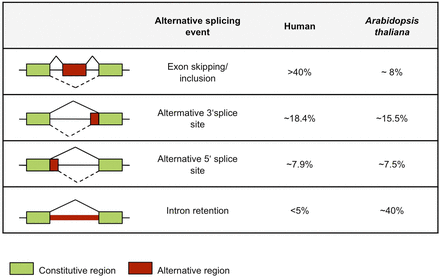
\includegraphics[width=.5\textwidth]{reddy-fig1}
        \caption{Reddy (2013) \cite{reddy_complexity_2013}}
      \end{figure}

      This may just be because Arabidopsis has such short introns. However it
      might be worth looking into how this affects orphan origins.

  \subsection{Exaption of transposon promoters}

    Many transposons are differentially regulated under stress.

    Transposon insertion into the non-exonic parts of genes may add stress
    resistence regulation or general upregulation (see Naito paper \cite{naito_unexpected_2009}).


  \subsection{Regulatory elements}

    Where do orphans get their regulatory elements? Chance?

    A nice review of plant orphans: \cite{priest_cis-regulatory_2009}.
    cis-regulatory elements coopoerate to create nuanced.

  \subsection{Papers}

    \subsubsection{Kapranov (2007) Genome-wide transcription and the
    implications for genomic organization}

      Citation \cite{kapranov_genome-wide_2007}

      A Science review on genome wide transcription 

    \subsubsection{Nagalakshmi (2008) The transcriptional landscape of the
    yeast genome defined by RNA sequencing}

      Citation \cite{nagalakshmi_transcriptional_2008}

      Yeast transciptional landscape 

      ``We applied RNA-Seq to generate a high-resolution transcriptome
      map of the yeast genome and demonstrated that most (74.5\%) of the
      nonrepetitive sequence of the yeast genome is transcribed''

    \subsubsection{Xu (2009) Bidirectional promoters generate pervasive
    transcription in yeast}
    
      Citation \cite{xu_bidirectional_2009}

    \subsubsection{Naito (2009) Unexpected consequences of a sudden and
    massive transposon amplification on rice gene expression}

      In a study by Naito (2009) \cite{naito_unexpected_2009}, the DNA
      transposon mPing was found to be proliferating in the rice strain EG4
      at a rate of about 40 jumps per generation. The TE preferentially
      jumped into genic, but not exonic, sequence. They usually upregulated
      the genes or did nothing. 156/710 showed difference in regulation, of
      these 111/156 were upregulated. 

      \begin{figure}[!hbpt]
        \centering
        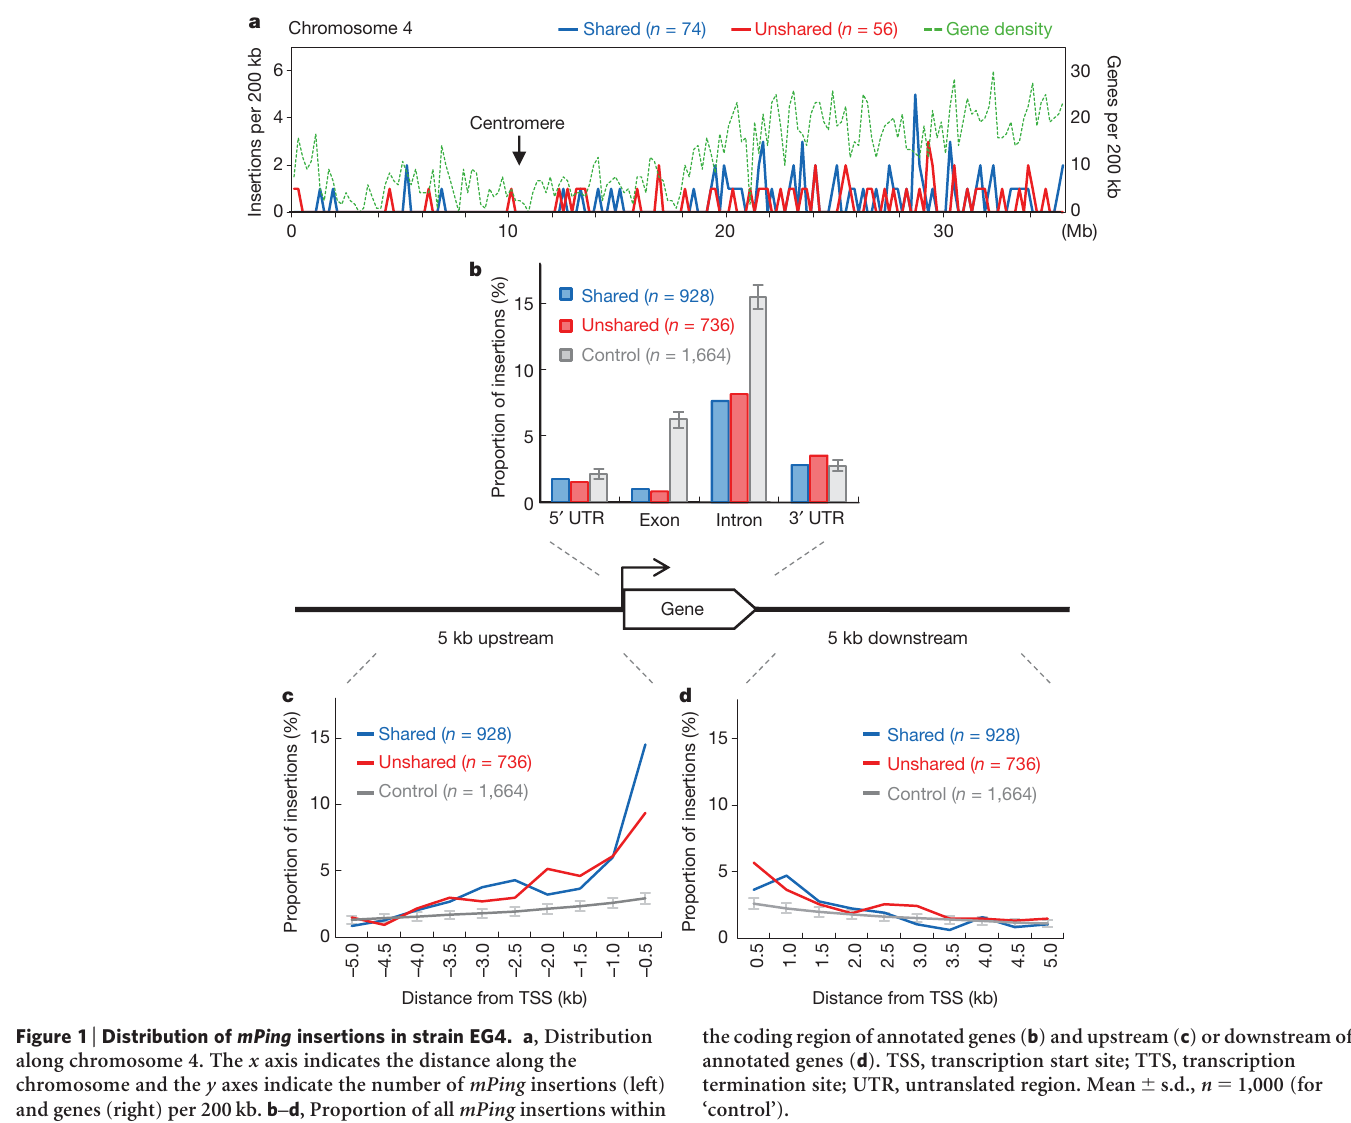
\includegraphics[width=\textwidth]{naito-transposons-2009-fig1}
        \caption{Naito (2009) \cite{naito_unexpected_2009}}
      \end{figure}

      \begin{figure}[!hbpt]
        \centering
        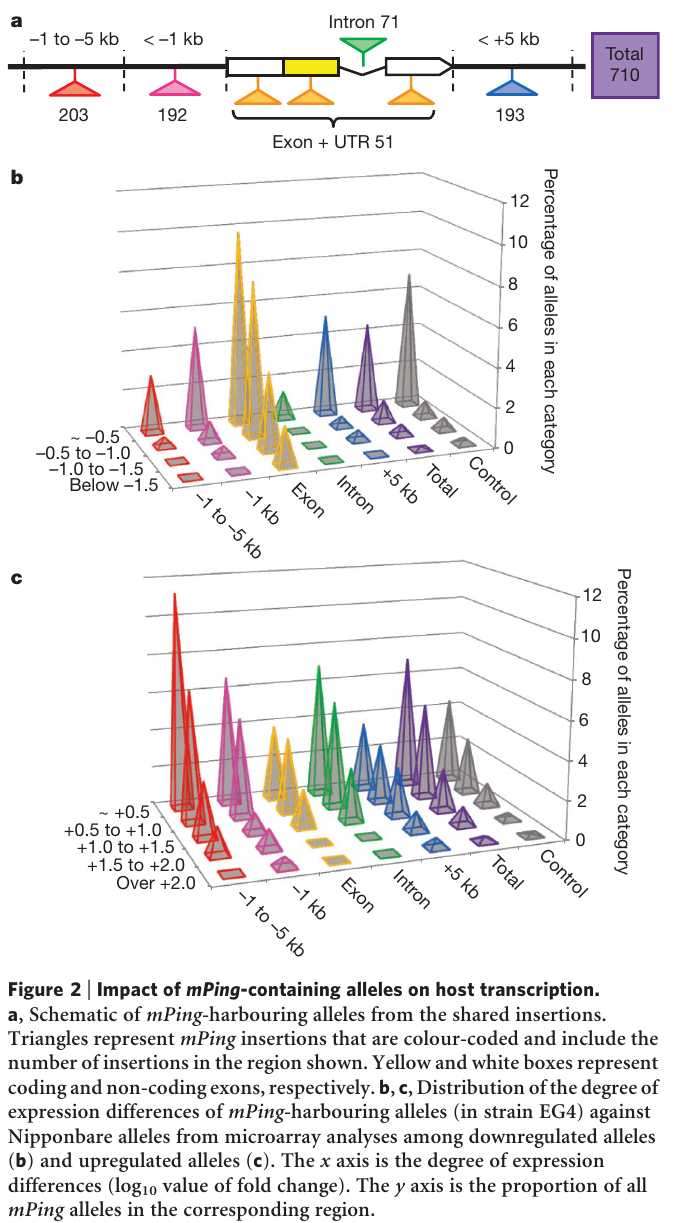
\includegraphics[height=0.7\textheight]{naito-transposons-2009-fig2}
        \caption{Naito (2009) \cite{naito_unexpected_2009}}
      \end{figure}
      \FloatBarrier

    \subsubsection{Haudry (2013) An atlas of over 90,000 conserved
    noncoding sequences provides insight into crucifer regulatory regions}

      Citation \cite{haudry_atlas_2013}

      They sequence three new crucifers: \textit{Leavenworthia alabamica},
      \textit{Sisymbrium irio} and \textit{Aethionema arabicum}.

      Performs an alignment of 9 Brassicaceae genomes, identifying
      conserved regions.



\section{Clade-specific factors}

\subsection{Transposon activity}

    Plants have very high transpson counts.

\subsection{Deletion rates}

    Plants have a much stronger gene deletion bias than mammals
    \cite{freeling_fractionation_2012}. Plants require such efficient gene
    removal mechanisms to reduce their gene set following polyploidy events
    \cite{thomas_following_2006, woodhouse_following_2010}. In contrast garbage
    can chill in mammalian genomes for millions of years (for example not one
    of the 200 dead genes in the human lineage have been deleted, rather they
    lay about as pseudogenes \cite{schrider_all_2009}).  For mammals orphans
    might be explained away as useless relics that the organisms has bothered
    to delete, but this is not the case in plants.  Therefore orphans may face
    harsher pressure, if they don't quickly become essential, they will be
    deleted. For this reason I would predict a more rapid rise to essentiality
    in plants than in mammals.

\subsection{Copy-variant appearance rate}

    Pretty high in plants and animals. A few percent in humans
    \cite{check_human_2005}. In a sequencing project of 80 \textit{Arabidopsis
    thaliana} accessions, there were about 444 genes absent in each accession
    ($~5\%$) \cite{tan_variation_2012}.

\section{Clues}

\subsection{Selective pressure is not strongly correlated with essentiality}

    This has been known for some time and incited much debate. 

\subsection{Selective pressure IS strongly correlated with expression}

    


\section{Reviews}
\subsection{Capra (2013) How old is my gene?}
    Citation \cite{capra_how_2013}

    A wonderful review dealing with many of my beefs with phylostratigraphy.
    Capra is a hardcore, algorithm and phylogenetics nerd. A real Liberles. He
    describes two parsimony methods: 1) Dollo parsimony, gain-loss gig where
    the MRCA is calculated allowing many losses but only one gain
    (phylostratigraphy is an example) and 2) Wagner parsimony, which places
    weights on different events. He argues that phylogenetic reconciliation
    should be used rather than naive phylostratigraphy.

    \begin{figure}[!hbpt]
        \centering
        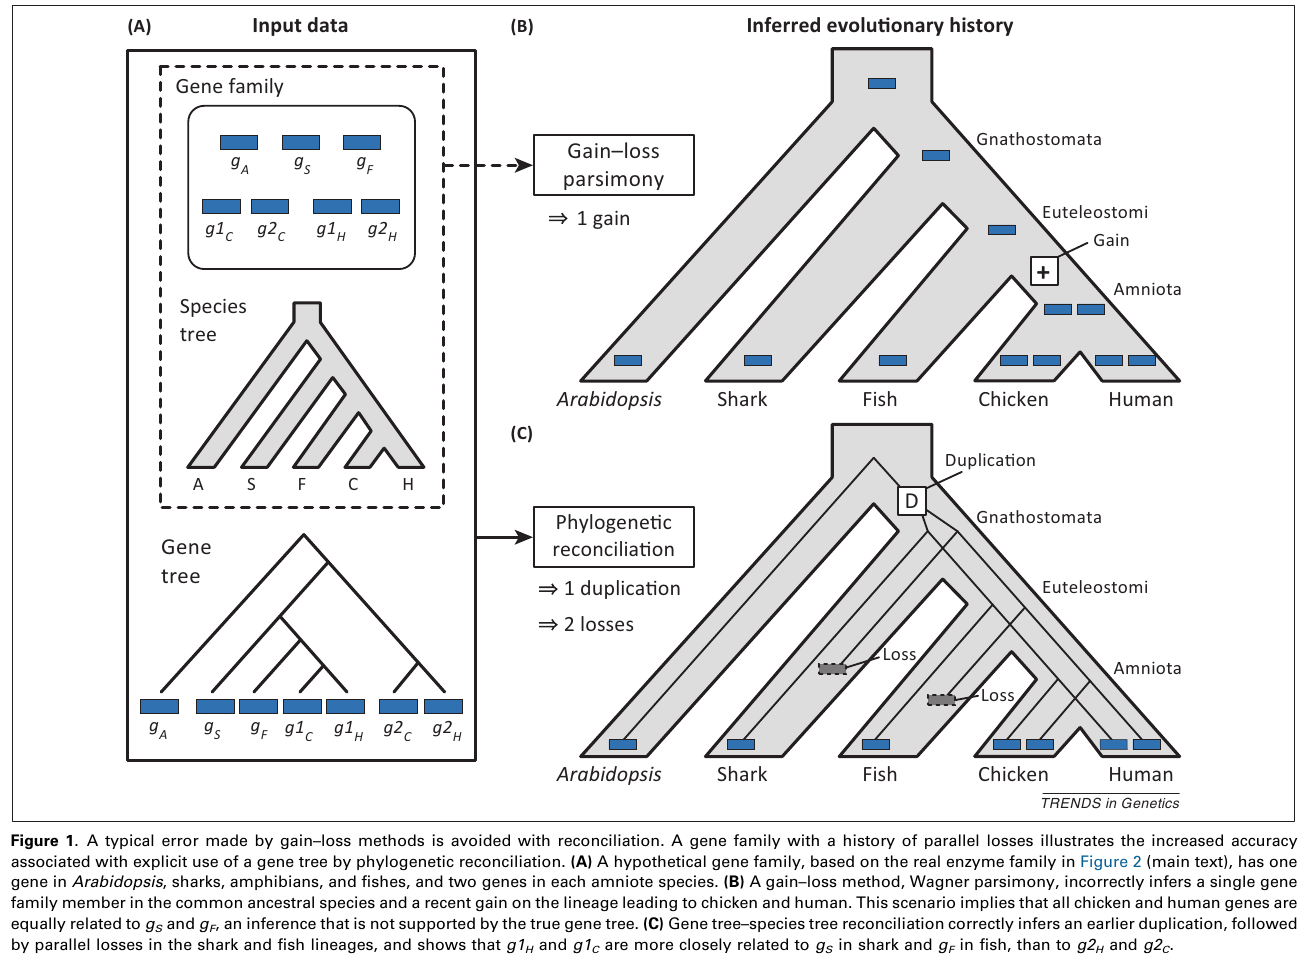
\includegraphics[width=0.9\textwidth]{capra-reconciliation-2013-fig1}
        \caption{Capra (2013) \cite{capra_how_2013}}
    \end{figure}
    \FloatBarrier

    \begin{figure}[!hbpt]
        \centering
        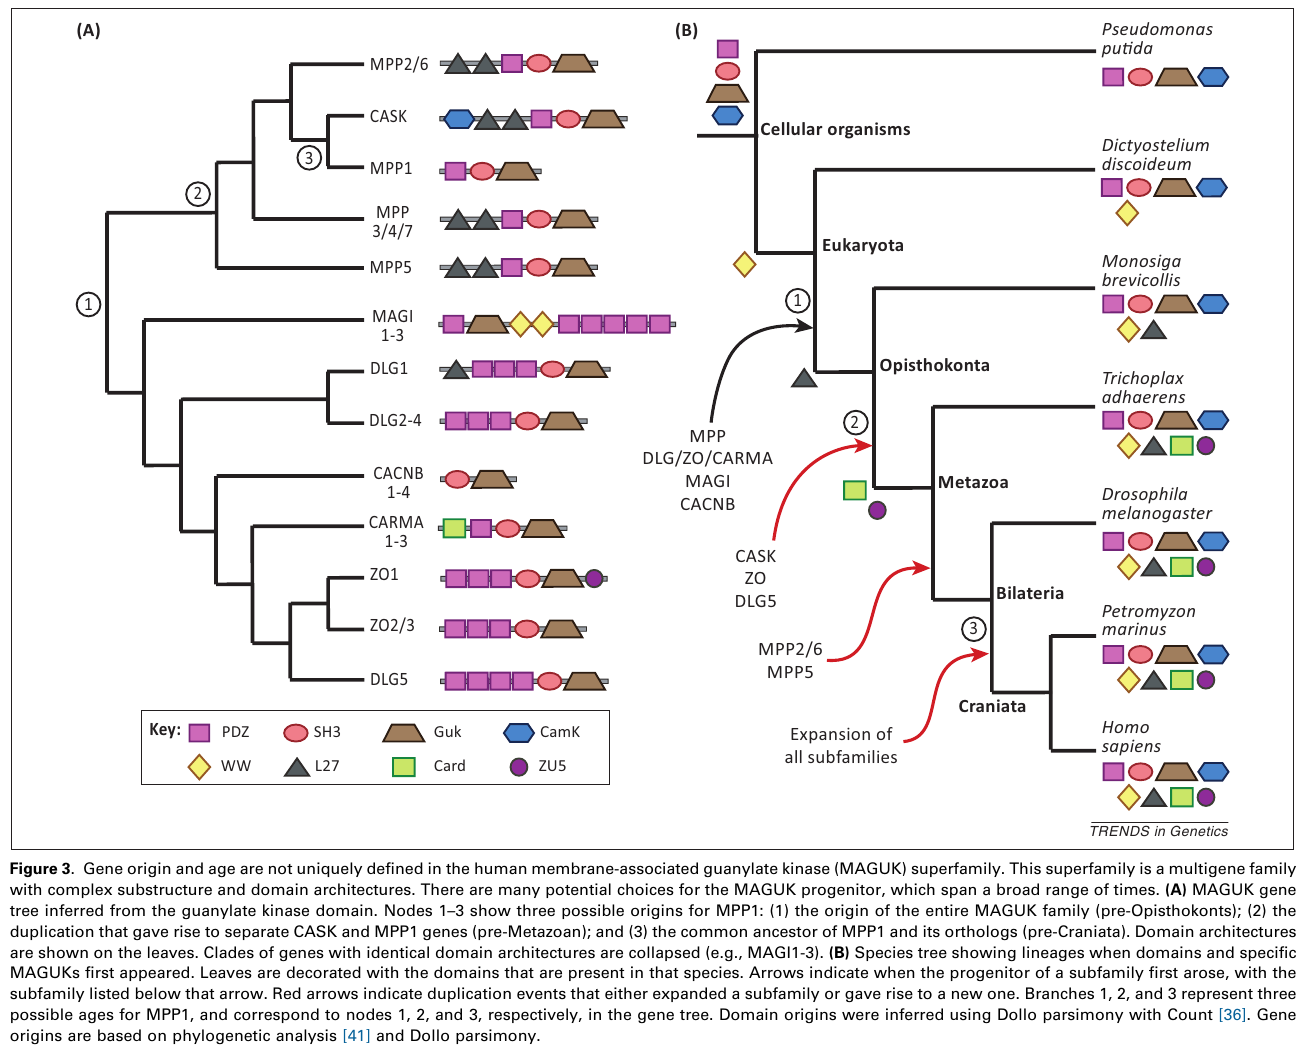
\includegraphics[width=0.9\textwidth]{capra-reconciliation-2013-fig3}
        \caption{Capra (2013) \cite{capra_how_2013}}
    \end{figure}
    \FloatBarrier

    Another problem is that major strata cannot be accurately dated

    \begin{figure}[!hbpt]
        \centering
        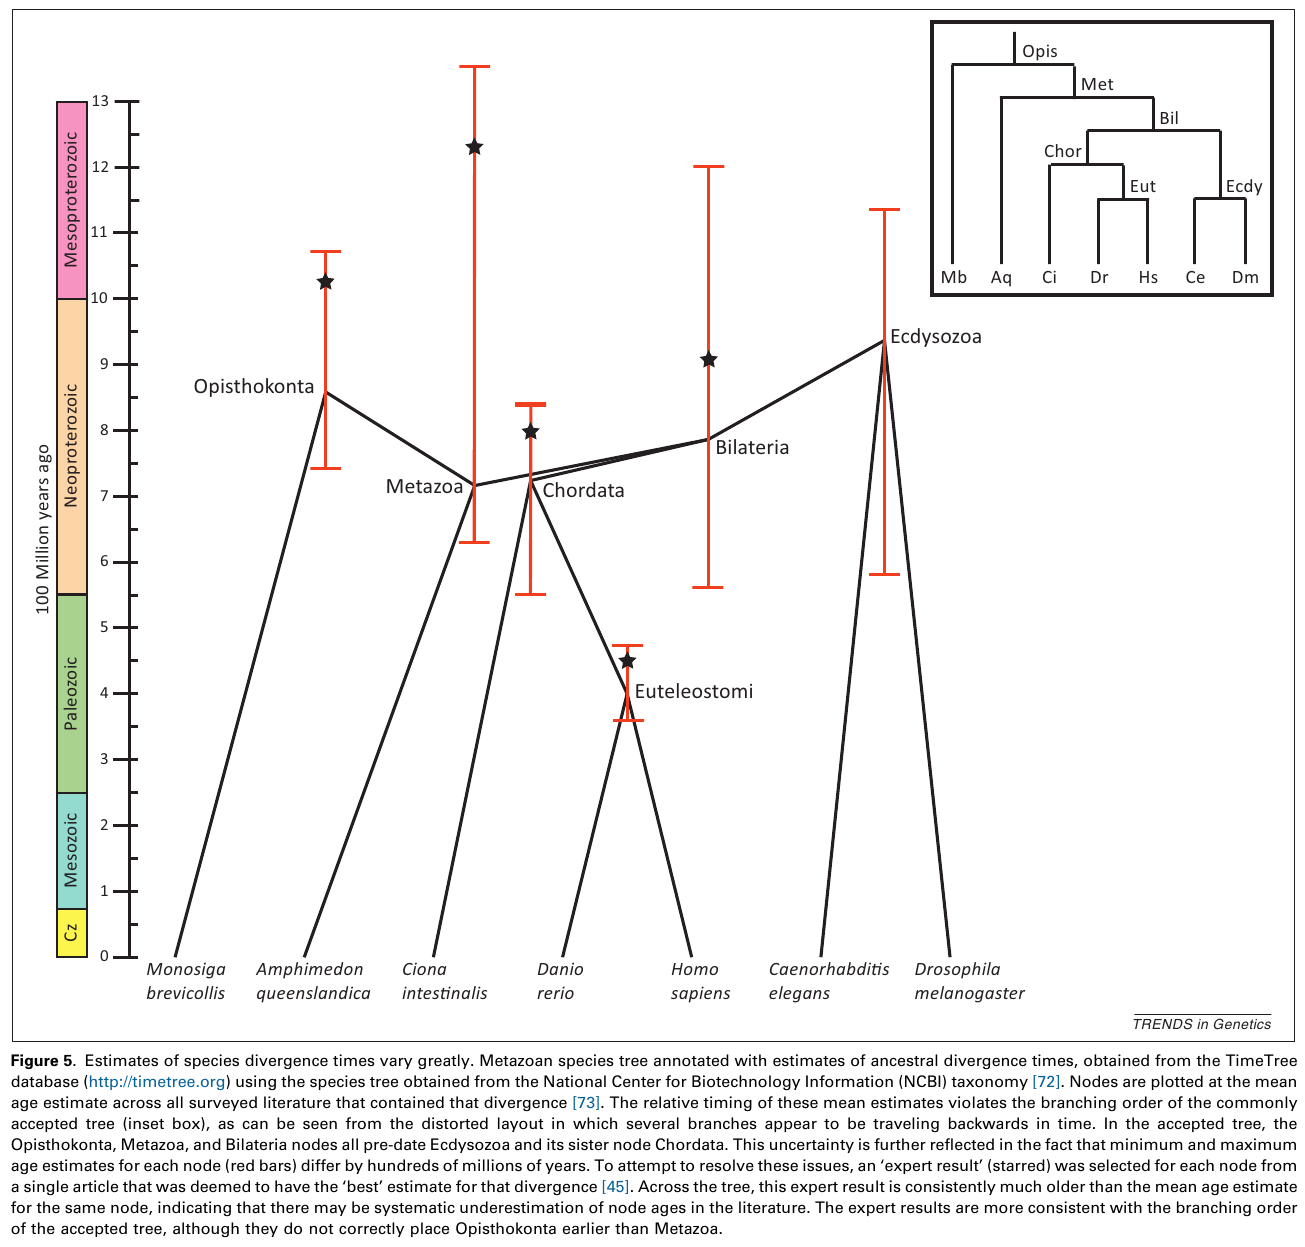
\includegraphics[width=0.9\textwidth]{capra-reconciliation-2013-fig5}
        \caption{Capra (2013) \cite{capra_how_2013}}
    \end{figure}
    \FloatBarrier

\subsection{Long (2013) New Gene Evolution: Little Did We Know}
    Citation \cite{long_new_2013}

    A very large (rather dry) review of the origins of new genes

\subsection{Lisch (2012) How important are transposons for plant evolution?}
    Citation \cite{lisch_how_2012}
    
    \begin{description}
        \item[Inactivate genes] Fairly pedestrian behavior, jump into a gene and disrupt it.
        \item[Reprogram gene expression] The simplest behvior is jumping into a
            promoter and disrupting it. However TEs have their own regulatory
            machinery, and often this can be used by the host gene. For example
            in the induction of stress regulation.
        \item[Delete, rearrange, transpose] 
        \item[Exapt coding sequence]
        \item[Epigenetics]
    \end{description}

\subsection{Bornberg-bauer (2013) Dynamics and adaptive benefits of modular
protein evolution}

    Citation \cite{bornberg-bauer_dynamics_2013}

    Claims $~80\%$ of rearangements are due to fusion, duplication and domain
    loss. The other things, exon shuffling etc, are less common.

    \begin{figure}[!hbpt]
        \centering
        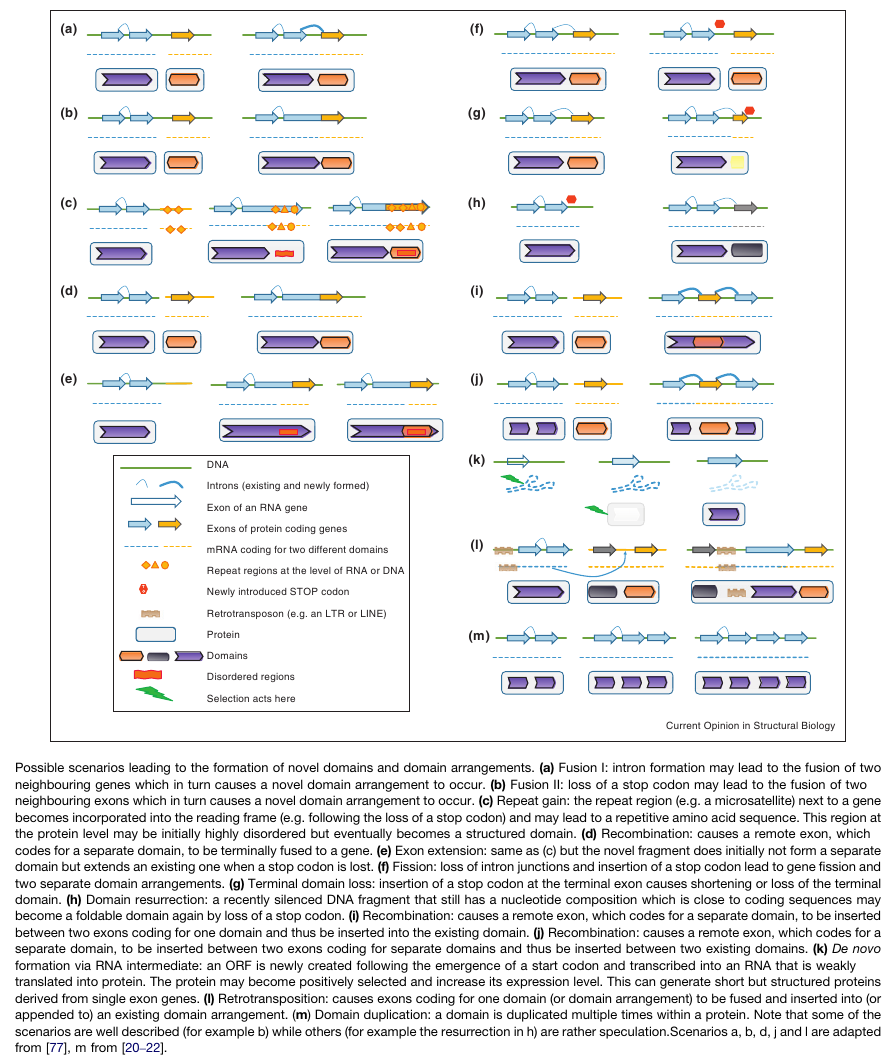
\includegraphics[height=0.7\textheight]{bornberg-bauer-2013-fig1}
        \caption{Bornberg-bauer (2013) fig1}
    \end{figure}
    \FloatBarrier

\subsection{Wu (2013) Evolution and function of de novo
originated genes}

    Citation \cite{wu_evolution_2013}

    ``Adaption following neutrality''

    Has a nice summary of the support for frequent \textit{de novo}
    proteogenesis. In both humans and drosophila, about 10\% of genes are
    \textit{de novo}.

    Mentions \textit{de novo} rise of RNAs, miRNA rise \textit{de novo} and
    by dulication at similar rates.

    States that orphans mainly rise \textit{de novo} (Khalturin et al.,
    2009; Tautz and Domazet-Loso, 2011)

    Orphan genes in animals are biased towards testes origin (many sources)

    \textit{De novo} genes are biased in humans towards brain tissue
    (several sources)

    States that little is known about function, mostly just ``guilt by
    association''.

    Neutral step then adaptive step (somewhat based off Carvunis):
\begin{enumerate}
    
    \item Neutral
    
        \begin{enumerate}
            
            \item Non-specific transcription
            \item Evolution of translateable ORF
            \item Selectable promiscuity - supported by the promiscuous
                orphan BSC4 in Sc \cite{cai_novo_2008}

        \end{enumerate}
        
    \item Adaptive
    
        \begin{enumerate}
            
            \item New gene is lifted by selection
            \item Rapid rise to importance by positive selection
        
        \end{enumerate}

\end{enumerate}

\subsection{Chen (2013) New genes as drivers of phenotypic evolution}

    Citation \cite{chen_new_2013}

    Describes the roles of orphans in metazoans.

    Keypoints: new genes rapidly gain new functions and become essential.

    New genes tend to gain roles in development, reproduction
    (spermatogenesis specifically), brain function and behaviour

    Discusses evolution of novel pathway via duplication in At (pp. 3)
    CYP98A

    New genes are needed in areas of rapid change. Resistance to stresses
    of changing environment, immune system in animals.

    Is spermatogenesis exceptional? Are there any search biases? Searching
    under streetlight?

    Artarctic fish antifreeze de novo proteins, required to deal with the
    new environment.

    ``The combination of phylostratigraphy and stage-specific gene
    expression data has revealed that the phylotypic stage expresses a
    transcriptome set representing older genes, whereas earlier and later
    developmental phases express relatively younger gene sets, in support
    of the hourglass mode \cite{kalinka_gene_2010,
    domazet-loso_phylogenetically_2010}''

    Chen doesn't mention it, but this hourglass trend has been confirmed in
    \textit{A. thaliana} as well \cite{quint_transcriptomic_2012}

    Most new essential genes are regulating early or late development.

\subsection{Ding (2012) Origins of New Genes and Evolution of Their Novel
Functions}

    Citation \cite{ding_origins_2012}
    
    Retrogenes: intronless and promoterless - pick up functions in
    spermatogenesis, courtship, ummunological response and brain

    Thought: retrogenes and orphan genes have similar functional patterns?

    ``The first straightforward search for de novo genes at the genome
    level was performed by Levine et al. (2006) in Drosophila'' pp. 9

    \textbf{Definitions of orphan genes: 1) genes without homologs 2) genes
    without homologs AND with synteny support.}

    ``Given these results together with other case studies, some common
    features of de novo genes are emerging. For example, these genes are
    relatively simple in intron/exon structure and tend to encode short and
    poorly structured proteins (Begun et al. 2006, Levine et al. 2006,
    Begun et al. 2007, Knowles \& McLysaght 2009).'' pp. 9

    There may be an ncRNA intermediate state between junk and orphan.

    ``Considering the abundance of lncRNAs in mammals and other eukaryotes
    (Mercer et al. 2009, Ponting et al. 2009), the above observations are
    particularly illuminative in suggesting the potential of lncRNAs to
    serve as a rich resource for de novo genes However, de novo genes may
    also evolve directly from noncoding DNA, as supported by the example of
    MDF1, whose orthologous loci are not expressed in the out-group species
    (Li et al. 2010b).'' pp. 10


    Chen et al. (2010) identified 566 young D. melanogaster genes that
    originated within 3–35 million years and systematically tested their
    phenotypic effects by RNA interference. Surprisingly, they found that
    30\% of these genes are essential for viability, which is comparable to
    that estimated for all genes in D. melanogaster (∼25–35\%)

\subsection{Ding (2012) Origins of New Genes and Evolution of Their Novel
Functions}

    Citation \cite{ding_origins_2012}
    
    Retrogenes: intronless and promoterless - pick up functions in
    spermatogenesis, courtship, ummunological response and brain

    Thought: retrogenes and orphan genes have similar functional patterns?

    ``The first straightforward search for de novo genes at the genome
    level was performed by Levine et al. (2006) in Drosophila'' pp. 9

    \textbf{Definitions of orphan genes: 1) genes without homologs 2) genes
    without homologs AND with synteny support.}

    ``Given these results together with other case studies, some common
    features of de novo genes are emerging. For example, these genes are
    relatively simple in intron/exon structure and tend to encode short and
    poorly structured proteins (Begun et al. 2006, Levine et al. 2006,
    Begun et al. 2007, Knowles \& McLysaght 2009).'' pp. 9

    There may be an ncRNA intermediate state between junk and orphan.

    ``Considering the abundance of lncRNAs in mammals and other eukaryotes
    (Mercer et al. 2009, Ponting et al. 2009), the above observations are
    particularly illuminative in suggesting the potential of lncRNAs to
    serve as a rich resource for de novo genes However, de novo genes may
    also evolve directly from noncoding DNA, as supported by the example of
    MDF1, whose orthologous loci are not expressed in the out-group species
    (Li et al. 2010b).'' pp. 10


    Chen et al. (2010) identified 566 young D. melanogaster genes that
    originated within 3–35 million years and systematically tested their
    phenotypic effects by RNA interference. Surprisingly, they found that
    30\% of these genes are essential for viability, which is comparable to
    that estimated for all genes in D. melanogaster (∼25–35\%)

\subsection{Khalturin (2009) More than just orphans: are
taxonomically-restricted genes important in evolution?}

    Citation \cite{khalturin_more_2009}

    A very coherent paper with a nice history or orphan genes. Covers only
    the animal side of things (with references to reasearch in bacteria).
    Focuses on cnidarian-specific genes.

    ``if the key developmental control genes are the same, and if conserved
    gene families serve similar functions in different organisms, how is
    the enormous morphological and physiological diversity within the
    animal kingdom generated?''

    Common answer: changes in regulation of these components ``rewiring''.

    \textbf{Comments on the 10-20\% orphan assertion:}

    States a 10-20\% figure for orphan composition across Eukaryota, based
    on 30 published genomes, 12 of which are Drosophilan
    \cite{clark_evolution_2007}. For some reason, he cites a 2000 paper for
    \textit{D. melanogaster} which reports 18\% or genes are orphan.
    However the 2007 paper, with the 12 genomes, reports only ~3\%. The
    genome paper suggests that many of the genes in the non-melanogaster
    genomes that were classified as being species-specific may be
    artefacts.

    Some of his other numbers I also really don't trust. Some of the
    genomes are separated by vast times (e.g. \textit{Tunicus intestinalis}
    is the sole sequenced genome in the Tunicata subphylum;
    \textit{Pristionchus pacificus} is 200 million years diverged from its
    nearest sequenced relative).
    
    His reports 11\% for rats, correctly citing the Nature rat genome paper
    \cite{gibbs_genome_2004}.  They report 10-11\% of rat proteins have no
    counterpart in humans.  \textbf{interesting sidenote:} This paper also
    says that there are 2302 rodent specific \textbf{exons} (shared in
    mouse and rat but absent in human).  Further actually the rat genome
    paper states that ``thirty-one Ensembl rat genes were collected that
    have no non-rodent homologues in current databases''. Interestingly,
    this implies a great proliferation of new genes since rats branched
    from mice, but very few of the de novo genes since the branch from
    humans have survived. As the paper says, these older de novo genes may
    have been incorporated as exons in extant genes.

    He cites a 2001 paper saying that 7\% of human genes are orphans,
    however the currnt estimate is only around 1\%.

    Overall, I really don't really trust his estimate. 

    \textbf{End of 10-20\% orphan assertion complaints}

    41 out of 50 nematocyte specific proteins are cnidarian-specific.
    \cite{hwang_evolutionary_2007}

    Basically, orphans were heavily recruited in the development of
    nematocytes. They played a role as structural componenets and
    developmental regulators.

    Most of their antimicrobial peptides show no homology. This doesn't
    really impress me. The peptides are short and necessarily change
    quickly (arms race). Aurelin is an example. Other examples exist in
    other lineages. Many very short, understudied?




\subsection{Stergiopoulos (2009) Fungal Effector Proteins}

    Citation \cite{stergiopoulos_fungal_2009}

    A voluminous review of fungal effectors. Often these effectors in fungal
    pathogens lack homology, possibly recruiting from orphans?

\subsection{Tautz (2011) The evolutionary origin of orphan genes}

    Citation \cite{tautz_evolutionary_2011}

    ``We propose that orphan genes continuously arise in any genome and
    that, at least in eukaryotes, they arise mostly through de novo
    evolution; however, we also propose that only a fraction of them
    assumes a long-term role in their respective evolutionary lineage,
    mainly in the context of evolutionary radiations'' pp. 1

    Provides rationale for trusting BLAST results. pp. 2

    Asserts gene shuffling is a minor factor citing \cite{}

\subsection{Gollery (2007) POFs: what we don’t know can hurt us}

    Citation \cite{gollery_pofs:_2007}

    Gollery phrases the issue in terms of what is unknown. He very
    specifically wants to summarize and understand the extent of our
    ignorance. The concept of POFs and PUFs are relavent to those seeking
    to delinieate the unknowneome. Orphans are differant. The orphan
    community is more interested in the novelty, the evolutionary rise,
    than the relative ignorance. Given the difference in usage, I don't
    think the terms should be merged. Gollery seeks a definition of the how
    unknown a protein is.

    While POF and orphan membership may heavily overlap, their definitions
    are quite different. POFs are defined relative to our ignorance,
    whereas orphans exist independently, being simply young genes.

    \begin{figure}[!hbpt] \centering
        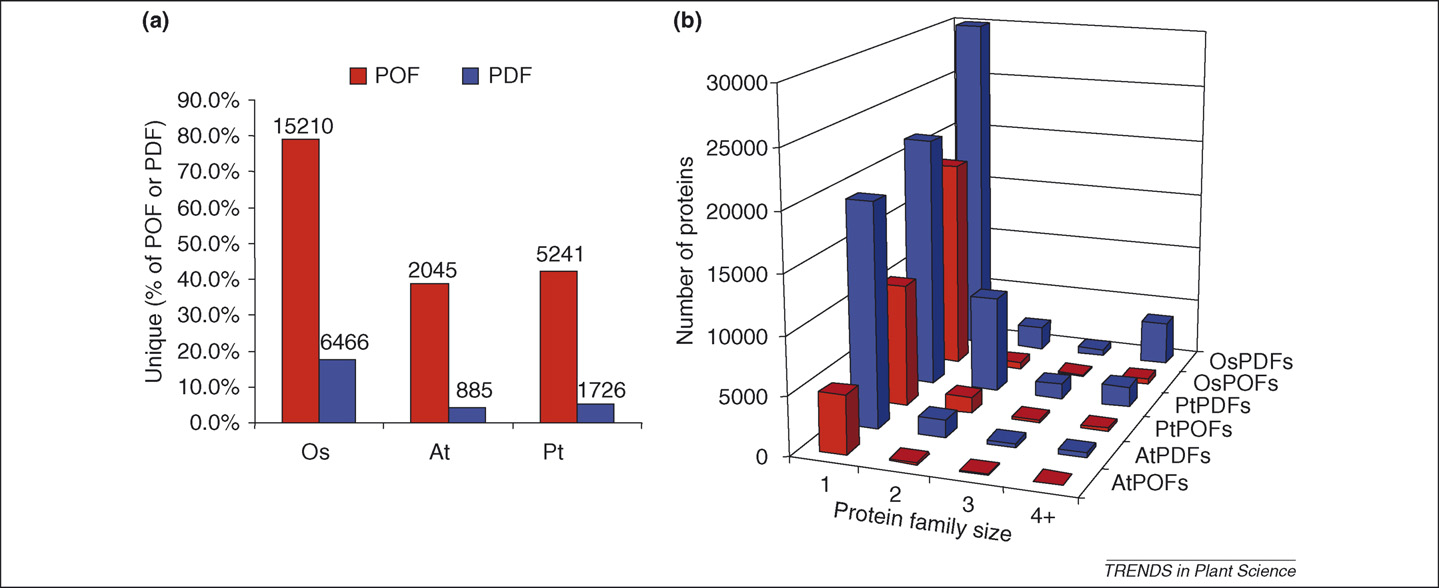
\includegraphics[scale=0.3]{gollery_hurt_2007-fig2}
        \caption{Gollery (2007) fig2} \end{figure} \FloatBarrier

\section{Papers}
\subsection{Neme (2013) Phylogenetic patterns of emergence of new genes
support a model of frequent de novo evolution}

    Citation \cite{neme_phylogenetic_2013}

    Uses phylostratigraphy to analyze trends across metazoans. A very
    powerful paper that does some of the same analyses I have done in At,
    which makes it a very nice source of comparisons.

    ``Younger genes are shorter, both with respect to gene length, as well
    as to open reading frame length. They contain also fewer exons and have
    fewer recognizable domains. Average exon length, on the other hand,
    does not change much over time'' pp. 1

    ``Conclusions: We suggest that the overall trends of gene emergence are
    more compatible with a de novo evolution model for orphan genes than a
    general duplication-divergence model. Hence de novo evolution of genes
    appears to have occurred continuously throughout evolutionary time and
    should therefore be considered as a general mechanism for the emergence
    of new gene functions.'' pp. 1

    ``With respect to gene length, the de novo model would predict that
    younger genes should be shorter than older genes, since it is unlikely
    that complex protein sequences emerge de novo. Rather one would expect
    that they could increase in size over evolutionary time. In the
    duplication-divergence model one would not expect length-dependence
    over time, since long and short genes should be equally likely subject
    to duplication at any time level.'' pp. 2.
    
    I do not agree. Long genes, if duplicated, would be more likely to have
    some region retain homology. If an ancient gene is duplicated and one
    daughter subsequently enters a period of neutral selection, her
    homology to her cousins will gradually decrease making her appear (to
    the phylostratigrapher) increasingly young, a Merlin effect). Assuming
    uniform mutation rates, a shorter gene will tend to reverse age more
    quickly.

    I further disagree with his reason for thinking de novo genes will be
    short. Of course it is true that specific information is not likely to
    appear by chance, but this is irrelevant. The length of monoexonic de
    novo proteins is determined by the distance between the start and stop
    codon.  This distance is distributed as a geometric random variable
    with a rate constant equal to the probability that a given codon is a
    stop codon. For polyexonic, cryptic de novo genes, length is determined
    by length and number of exons. Long polyexonic genes require multiple
    fortuitous events, thus are statistically unlikely to be long. Either
    way, length has nothing to do with protein complexity.

\subsection{Toll-riera (2013) Emergence of novel domains in proteins}

    Citation \cite{toll-riera_emergence_2013}

    Proteins are gradually lengthened by addition of young domains.

    ``\ldots we have identified all human young protein domains that have
    emerged in approximately the past 550 million years. \ldots We have
    found 426 different annotated young domains, totalling 995 domain
    occurrences, which represent about 12.3\% of all human domains. We have
    observed that 61.3\% of them arose in newly formed genes, while the
    remaining 38.7\% are found combined with older domains, and have very
    likely emerged in the context of a previously existing protein. Young
    domains are preferentially located at the N-terminus of the protein
    \ldots Furthermore, young domains show significantly higher
    non-synonymous to synonymous substitution rates than older domains
    using human and mouse orthologous sequence comparisons. This is also
    true when we compare young and old domains located in the same protein,
    suggesting that recently arisen domains tend to evolve in a less
    constrained manner than older domains. Conclusions: We conclude that
    proteins tend to gain domains over time, becoming progressively longer.
    We show that many proteins are made of domains of different age, and
    that the fastest evolving parts correspond to the domains that have
    been acquired more recently.'' pp. 1

    Genes in Eukaryotes tend to grow by addition of novel domains at the 3'
    (N-terminus) end.

    Apparently the way proteins gain domains has been thorougly studied
    \cite{chothia_evolution_2003, vogel_structure_2004,
    ekman_multi-domain_2005, moore_arrangements_2008,
    buljan_evolution_2009, marsh_how_2010, moore_dynamics_2011,
    ekman_quantification_2007}.

\subsection{Abrusan (2013) Integration of New Genes into Cellular Networks,
    and Their Structural Maturation} 

    Citation \cite{abrusan_integration_2013}

    ``I show that $1)$ The number of regulatory, protein–protein, and
    genetic interactions increases continuously with gene age, although
    with very different rates. New regulatory interactions emerge rapidly
    within a few million years, while the number of protein–protein and
    genetic interactions increases slowly, with a rate of 2-2.25 $\times$
    $10^{-8}$/year and 4.8 $\times$ $10^{-8}$/year, respectively. $2)$ Gene
    essentiality evolves relatively quickly: the youngest essential genes
    appear in proto-genes $\sim$14 MY old. $3)$ In contrast to
    interactions, the secondary structure of proteins and their robustness
    to mutations indicate that new genes face a bottle- neck in their
    evolution: proto-genes are characterized by high b-strand content, high
    aggregation propensity, and low robustness against mutations, while
    conserved genes are characterized by lower strand content and higher
    stability, most likely due to the higher probability of gene loss among
    young genes and accumulation of neutral mutations.'' pp. 1

    Builds off the Carvunis results.

    Sets out to test two things: $1)$ integration of orphans into networks
    $2)$ the continuity ngORF-protogene-gene continuity predicted by
    Carvunis.

\subsection{Wissler (2013) Mechanisms and Dynamics of Orphan Gene Emergence
in Insect Genomes} 

    Citation \cite{wissler_mechanisms_2013}

    Calculated the number of orphans in each of 30 insect genomes. Found an
    expected ~500 orphan genes per genome (~4\%). Of these, 43 \% for
    Formicidae species and 61\% for Attini species had matches to non-genic
    sequence.

    \cfig{scale=1}{wissler_insect_2013-fig2}{Wissler \textit{et al.} Insect tree}

    \cfig{scale=0.5}{wissler_insect_2013-fig1}{Wissler \textit{et al.} orphan
      count versus separation from nearest relative}

    \cfig{scale=0.2}{wissler_insect_2013-supfig5}{Wissler \textit{et al.} various traits}

\subsection{Thakur (2013) De Novo Transcriptome Sequencing and Analysis for
Venturia inaequalis, the Devastating Apple Scab Pathogen}

    Citation \cite{thakur_novo_2013}

    \begin{description}
        \item[Set A] 24571 unique genes with homology. 463 putative secreted
            proteins.
        \item[Set B] 32311 assembled transcripts without homology. 483 putative
            secreted proteins.
    \end{description}

    \cfig{scale=1}{thakur_denovo_2013-fig4}{%
      Thakur \textit{et al.} (fig 4) \textbf{Set A} has homology,
      \textbf{Set B} doesn't.
    }

\subsection{Gibson (2013) Why so many unknown genes? Partitioning orphans
from a representative transcriptome of the lone star tick Amblyomma
americanum}

    Citation \cite{gibson_why_2013}

    EST based estimate of orphan percentages in ticks.

    ``Expressed sequence tags (ESTs) were derived from different life stages
    and populations of A. americanum and combined with ESTs available from
    GenBank to produce 14,310 ESTs, over twice the number previously available.
    The vast majority (71\%) has no sequence homology to proteins archived in
    UniProtKB. We show that poor sequence or assembly quality is not a major
    contributor to this high representation by orphan genes. Moreover, most
    unannotated sequences are functional: a microarray experiment demonstrates
    that 59\% of functional ESTs are unannotated. Lastly, we attempt to further
    annotate our EST dataset using genomic datasets from other members of the
    Acari, including Ixodes scapularis, four other tick species and the mite
    Tetranychus urticae. We find low homology with these species, consistent
    with significant divergence within this subclass'' pp. 1

    ``We conclude that the abundance of orphan genes in A. americanum likely results
    from 1) taxonomic isolation stemming from divergence within the tick lineage
    and limited genomic resources for ticks and 2) lineage- specific genes needing
    functional genomic studies to evaluate their association with the unique
    biology of ticks.  The EST sequences described here will contribute
    substantially to the development of tick genomics. Moreover, the framework
    provided for the evaluation of orphan genes can guide analyses of future
    transcriptome sequencing projects.'' pp. 1

    Cites transcriptome projects from 12 mite species [hers, 24-35].

    71\% figure seems ridiculous, as the author is keenly aware. She discusses
    the problems. Many of the orphans may be due to issues with annotation,
    especially in the nearset neighbor. Tentative. More certainty requires a
    full transcriptome.

\subsection{Carvunis (2012) Proto-genes and de novo gene birth}

    Citation \cite{carvunis_proto-genes_2012}

    Introduces ngORF to proto-gene to mature gene model. Uses RNA-seq data
    as evidence of ORF transcription and ribosome footprinting as evidence
    of translation.

    proto-gene := transcribed AND translated ORF
    
    ``Such a reservoir of proto-genes would allow evolutionary innovations
    to be attempted without affecting existing genes'' pp. 1

    \cfig{scale=0.6}{carvunis_protogene-fig1}{%
      Carvunis (2012) protogenes and trees. Top right, number of ORFs assigned
      to each conservation level (logarithmic scale). A.  gossypii, Ashbya
      (Eremothecium) gossypii; A. nidulans, Aspergillus nidulans; C. albicans
      (Saccharomycetales MRCA 490 mya), Candida albicans; D. hansenii,
      Debaryomyces hansenii; K.  lactis, Kluyveromyces lactis; K. waltii,
      Kluyveromyces (Lachancea) waltii; N. crassa, Neurospora crassa; S. pombe,
      Schizosaccharomyces pombe (Ascomycota MRCA ~800 mya).
    }

    \cfig{scale=0.6}{carvunis_protogene-fig2}{%
      Carvunis (2012) trends in yeast \cite{carvunis_proto-genes_2012}.  ~14
      million year spread between first 4 strata, ~800 million years from
      strata 10.
    }

    \cfig{scale=0.6}{carvunis_protogene-fig3}{%
      Carvunis (2012) ribosome binding, AUG optimal context, purifying
      selection, stress   
    }

    Trends:

    \begin{enumerate}
        
        \item Increase in intrinsic disorder

        Disorder increases early, peals at a stratum ~490 mya, then falls.

        In At, the disorder jumps from low in ngORFs to high in orphans,
        remains steady, then falls significantly in the Viridiplantae and
        Eukaryota strata.

        \item Increase in codon optimization \item Increase in RNA abundance
    \item Increase in nearby transcription factor binding sites \item
    Increase in length \item Decrease in hydropathicity \end{enumerate}

    All of these, except transcription factors and hydropathicity, I have
    confirmed in \textit{A. thaliana}


\subsection{Colbourne (2011) The Ecoresponsive Genome of Daphnia pulex}

    Citation \cite{colbourne_ecoresponsive_2011}

    \cfig{scale=0.6}{colbourne_daphnia_2011-fig5}{%
      Colbourne (2011) fig5 Daphnia pulex \cite{colbourne_ecoresponsive_2011}
    }

\subsection{Moore (2011) The Dynamics and Evolutionary Potential of Domain
Loss and Emergence}

    Citation \cite{moore_dynamics_2011}


\subsection{Buljan (2010) Quantifying the mechanisms of domain gain in animal proteins}
    Citation \cite{buljan_quantifying_2010}

    In animals, proteins usually grow by fusion with the exons of adjacent
    genes or exonization of non-genic sequence.

    \textbf{``Background: Protein domains are protein regions that are shared
        among different proteins and are frequently functionally and
        structurally independent from the rest of the protein. Novel domain
        combinations have a major role in evolutionary innovation. However, the
        relative contributions of the different molecular mechanisms that
        underlie domain gains in animals are still unknown. By using animal
        gene phylogenies we were able to identify a set of high confidence
        domain gain events and by looking at their coding DNA investigate the
        causative mechanisms.}

    \textbf{``Results: Here we show that the major mechanism for gains of new
        domains in metazoan proteins is likely to be gene fusion through
        joining of exons from adjacent genes, possibly mediated by non-allelic
        homologous recombination.  Retroposition and insertion of exons into
        ancestral introns through intronic recombination are, in contrast to
        previous expectations, only minor contributors to domain gains and have
        accounted for less than 1\% and 10\% of high confidence domain gain
        events, respectively.  Additionally, exonization of previously
        non-coding regions appears to be an important mechanism for addition of
        disordered segments to proteins. We observe that gene duplication has
        preceded domain gain in at least 80\% of the gain events.}

    \textbf{``Conclusions: The interplay of gene duplication and domain gain
        demonstrates an important mechanism for fast neofunctionalization of
        genes.''}

    \cfig{width=\textwidth}{buljan-domain-2010-fig1}{ Buljan (2010) }
    \cfig{width=\textwidth}{buljan-domain-2010-fig2}{ Buljan (2010) }
    \cfig{width=\textwidth}{buljan-domain-2010-fig3}{ Buljan (2010) }

    
\subsection{Gollery (2006) What makes species unique? The contribution of
proteins with obscure features}

    Citation \cite{gollery_what_2006}

\subsection{Ohno (1970) Evolution by gene duplication}

    Citation \cite{ohno_evolution_1970}

    Argues that new genes come almost exclusively from old genes. The idea
    is much older than this book, but Ohno is the oft cited champion of the
    idea.

\section{Plant papers}
\subsection{Ye (2013) Evolutionary analyses of non-family genes in plants}

    Citation \cite{ye_evolutionary_2013}

    The paper isn't focused at all on orphans. The main interest is (as the
    title suggests) non-family genes.

    \begin{description} \item[NF] non-family (1-2 per genome) \item[LF]
            low-copy family (3-10 per genome) \item[HF] high-copy family
                (>10 per genome \end{description}

    Cluster analysis on 14 plant genomes. Identifies rough strata. Counts
    strata-specific non-family (NF) genes. Arabidopsis thaliana is the only
    Brassicacea member.

    \begin{figure}[!hbpt] \centering 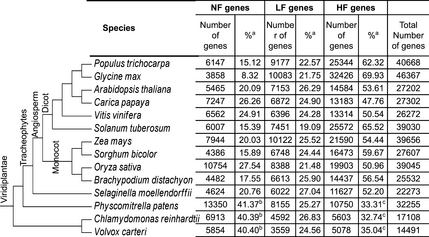
\includegraphics{ye_nonfamily-fig1}
        \caption{ ${}^b$ Lower plants have significantly ($P < 0.01$,
        Chi-square) higher proportion of NF genes than higher plants.
        ${}^c$ Lower plants have significantly ($P < 0.01$, Chi-square)
        lower proportion of HF genes than higher plants } \end{figure}

    \begin{figure}[!hbpt] \centering 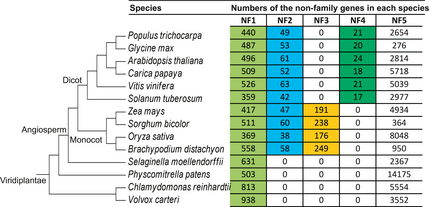
\includegraphics{ye_nonfamily-fig3}
        \caption{ Distribution of non-family (NF; 1 or 2 copies) genes
            among different phylogenetic groups. NF1 gene group contains NF
            genes having homologues in all the 14 species; NF2 contains NF
            genes having homologues in all and only the 10 angiosperm
            species; NF3 contains NF genes having homologues in all and
            only the four monocot species; NF4 contains NF genes having
            homologues in all and only the six dicot species; and NF5
            contains species-specific NF genes. The numbers of genes in
        each species were normalized based on Glycine, which has the
    highest number of genes among the 14 species studied.  } \end{figure}

    \begin{figure}[!hbpt] \centering 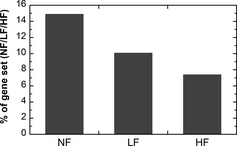
\includegraphics{ye_nonfamily-fig8}
        \caption{ Hub genes in non-family (NF; 1 or 2 copies),
            low-copy-number family (LF; 3-10 copies) and high-copy-number
            family (HF; $>$10 copies) sets. Hubs were defined here as the
            top 10\% most connected nodes in the Arabidopsis
        protein-protein interaction network } \end{figure} \FloatBarrier

\subsection{Guo (2013) Gene family evolution in green plants with emphasis
    on the origination and evolution of \textit{Arabidopsis thaliana}
genes}

\subsection{Freeling (2012) Fractionation mutagenesis and similar consequences
    of mechanisms removing dispensable or less-expressed {DNA} in plants}

    Citation \cite{freeling_fractionation_2012}

    Junk hangs out for millions of years in mammals, but flowering plants take
    out the garbage. For example, all 200 dead genes in the human lineage
    remain as pseudogenes \cite{schrider_all_2009}. However in plants maize
    \cite{woodhouse_following_2010} and Arabidopsis
    \cite{thomas_following_2006} extremely rapid loss of duplicated genes were
    found to follow tetraploidy events. The main mechanism is intra-chromosomal
    or illgenimate recombination \cite{woodhouse_following_2010}.

\subsection{Wang (2010) Evolutionary Transients in the Rice Transcriptome}

    Citation \cite{wang_evolutionary_2010}

    The tail of the degenerate twin

    ``In the canonical version of evolution by gene duplication, one copy
    is kept unaltered while the other is free to evolve. This process of
    evolutionary experimentation can persist for millions of years. Since
    it is so short lived in comparison to the lifetime of the core genes
    that make up the majority of most genomes, a substantial fraction of
    the genome and the transcriptome may—in principle—be attributable to
    what we will refer to as “evolutionary transients”, referring here to
    both the process and the genes that have gone or are undergoing this
    process. Using the rice gene set as a test case, we argue that this
    phenomenon goes a long way towards explaining why there are so many
    more rice genes than Arabidopsis genes, and why most excess rice genes
    show low similarity to eudicots.'' abstract, pp. 1

    
\subsection{Luhua (2008) Enhanced Tolerance to Oxidative Stress in Transgenic
Arabidopsis Plants Expressing Proteins of Unknown Function}

Citation \cite{luhua_enhanced_2008}

The study is focused on POFs (proteins of obscure function) rather than
orphans. But it identifies the rough strata of all of the POFs. This paper
is particularly important because it contains experimental verification of
several functional orphans.

Procedure: Identified 41 POFs that respond to oxidative stress and
expressed them constitutively in transgenic A. thaliana lines.

``We found that more than 70\% of the expressed unknown proteins conferred
tolerance to oxidative stress. In contrast, the majority of expressed
unknowns (.90\%) did not confer tolerance to the other stresses tested, and
approximately 50\% of the expressed un- known proteins rendered plants more
susceptible to osmotic or salinity stress'', pp. 2

At-specific loci:

\begin{description}

    \item[AT1G21520] l=66; BLAST(nr) genus-specific 

    \item[AT1G50290] l=134; BLAST(nr) species-specific (e-0.004 to lyrata)

    \item[AT1G64360] l=85; BLAST(nr) Camelineae-specific (strong match to
        Capsella). $~$6-fold upregulated under osmotic stress.
    
    \item[AT2G41650] l=66; BLAST(nr) species-specific. $~$2-fold
        upregulated under oxidative stress.
        
\end{description}

Brassica-specific loci: AT2G22080, AT5G18040

\begin{description}

    \item[AT2G22080] l=177; BLAST(nr) Zinc-finger domain. $~$15-fold
        upregulated under oxidative stress.

    \item[AT5G18040] l=; BLAST(nr)

\end{description}

Identifies 2 Arabidopsis specific and 1 Brassica-specific oxidative stress
tolerance enhancing genes.

\subsection{Armisen (2008) Unique genes in plants: specificities and
conserved features throughout evolution}

    Citation \cite{armisen_unique_2008}

    Based only on Arabidopsis and Oryza

    Focused on unique (as in single-family) genes, not specfically orphans.
    Orphans are genes with no orthologs, unique genes are those with no
    paralogs.

    ``Many of the A. thaliana and O. sativa unique genes are conserved in
    plants for which the ancestor diverged at least 725 million years ago
    (MYA). Half of these genes are also present in other eukaryotic and/or
    prokaryotic species. Thus, our results indicate that (i) a strong
    negative selection pressure has conserved a number of genes as unique
    in genomes throughout evolution, (ii) most unique genes are subjected
    to a low divergence rate, (iii) they have some features observed in
    housekeeping genes but for most of them there is no functional
    annotation and (iv) they may have an ancient origin involving a
    possible gene transfer from ancestral chloroplasts or bacteria to the
    plant nucleus.'' pp. 1

\subsection{Castellana (2008) Discovery and revision of Arabidopsis genes by proteogenomics}

    All based on TAIR7, TAIR8 does not incorporate their work and only 3\% of
    the novel genes Castellana finds are added to TAIR8. TAIR9 incorporated
    Castellana's results \cite{lamesch_arabidopsis_2011}.

    Castellana says genomics and proteomics people should be friends.

    Citation \cite{castellana_discovery_2008}

    ``Gene annotation underpins genome science. Most often protein coding
    sequence is inferred from the genome based on transcript evidence and
    computational predictions. While generally correct, gene models suffer from
    errors in reading frame, exon border definition, and exon identification.
    To ascertain the error rate of Arabidopsis thaliana gene models, we
    isolated proteins from a sample of Arabidopsis tissues and determined the
    amino acid sequences of 144,079 distinct peptides by tandem mass spectrom-
    etry. The peptides corresponded to 1 or more of 3 different translations of
    the genome: a 6-frame translation, an exon splice- graph, and the currently
    annotated proteome. The majority of the peptides (126,055) resided in
    existing gene models (12,769 con- firmed proteins), comprising 40\% of
    annotated genes. Surpris- ingly, 18,024 novel peptides were found that do
    not correspond to annotated genes. Using the gene finding program AUGUSTUS
    and 5,426 novel peptides that occurred in clusters, we discovered 778 new
    protein-coding genes and refined the annotation of an addi- tional 695 gene
    models. The remaining 13,449 novel peptides provide high quality annotation
    (>99\% correct) for thousands of additional genes. Our observation that
    18,024 of 144,079 peptides did not match current gene models suggests that
    13\% of the Arabidopsis proteome was incomplete due to approximately equal
    numbers of missing and incorrect gene models.'' abstract

    \begin{figure}[!hbpt]
        \centering
        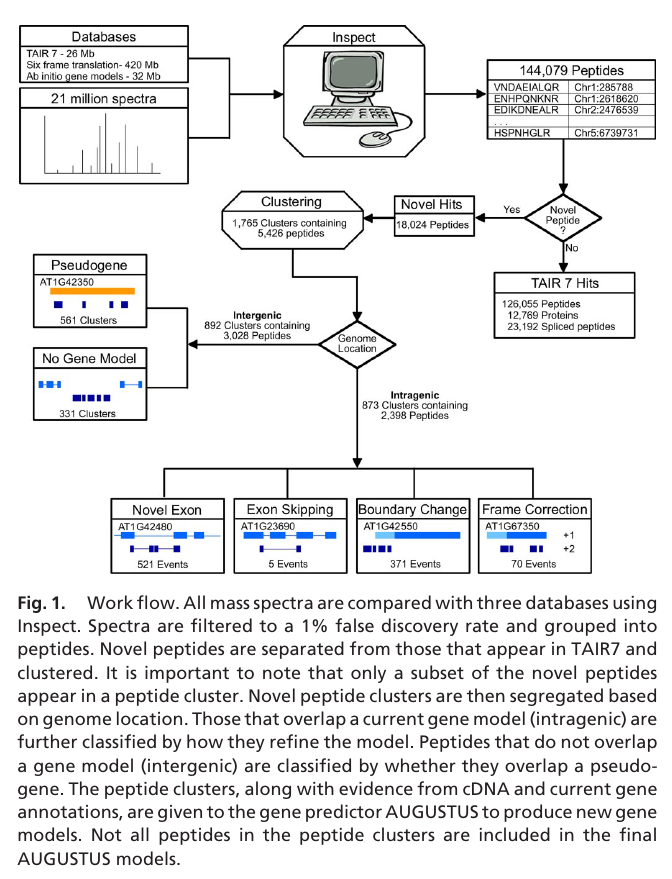
\includegraphics[width=0.5\textwidth]{castellana-2008-fig1}
        \caption{Castellana (2008) fig1}
    \end{figure}
    \FloatBarrier

\section{Genome Projects}
\subsection{Entelegyne Spider}

  Citation \cite{carlson_novo_2015}

  ``In this study, the transcriptomes of six entelegyne spider species from
  three genera (\textit{Cicurina travisae}, \textit{C. vibora},
  \textit{Habronattus signatus}, \textit{H. ustulatus}, \textit{Nesticus
    bishopi} and \textit{N.  cooperi}) were sequenced and de novo assembled
  \dots between ~ 400 and 1,100 unique orphan genes were found to be present in
  each congeneric lineage''

\subsection{Potato blight \textit{Phytophthora infestans}}

  Citation \cite{haas_genome_2009}

  Genome is arragned into two sets of blocks: 1) gene-rich, synteny-conserved
  blocks and 2) gene-poor, repeat-rich, TE-rich, and secreted-effector-rich
  blocks.

  $~$1/3 of the genome is comprised of Gypsy elements.

  Some fungal motifs effectors are conserved, such as the huge RXLR (563, half
  species-specific) and Crinkler (CRN) families of cytoplasmic effectors
  \cite{haas_genome_2009}. The RXLR effectors where identified via HMM against
  known motifs, however, at the unweighted sequence level, half were
  species-specific. Only 16/563 where present in all three sequenced species of
  the genus. These genes had extremely fast turnover rate. Markov clustering
  (TribalMCL) show 1 large family and 150 smaller ones. The RXLR genes are
  mostly in the gene-sparse blocks, where transposons can hasten evolution.

  CRN cytoplasmic effectors have a conserved N-terminal $~$50 aa LFLAK domain
  and highly variable C-terminal domain(s). They are concentrated in
  gene-sparse regions where they may rapidly recombine, shuffling the
  C-terminal domain into new sequences.

  The authors suggest non-allelic homologous recombination and tandem gene
  duplication as the primary methods of family expansion in RXLR and CRN.  They
  find no evidence of transposition.

  \begin{figure}[h!]
    \centering
    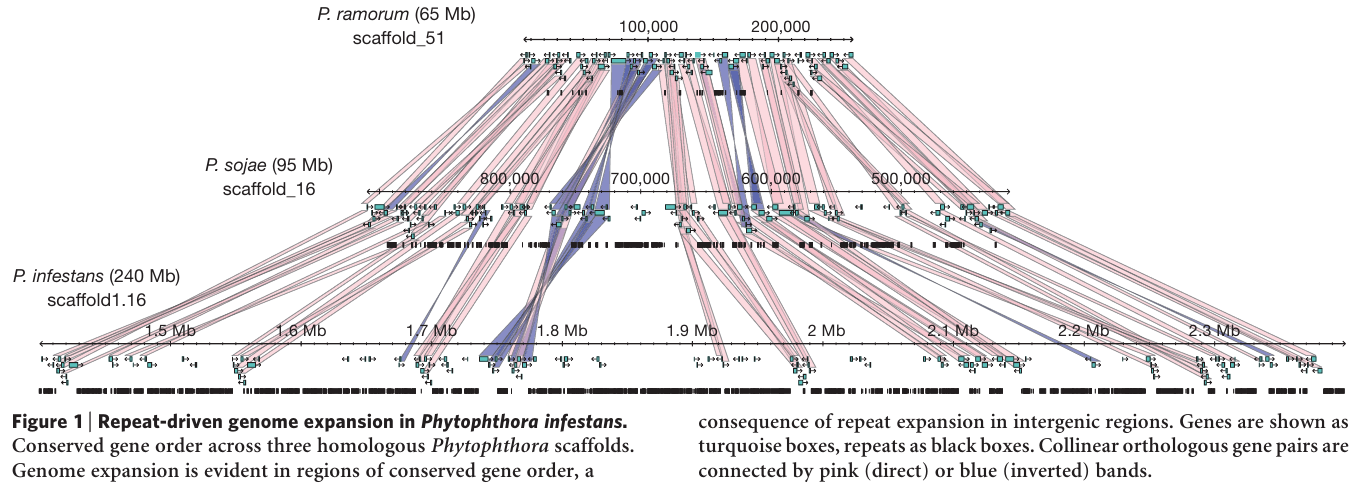
\includegraphics[width=\textwidth]{haas_blight_2009-fig1}
    \caption{
        Haas (2009) \cite{haas_genome_2009}
    }
  \end{figure}

  \begin{figure}[h!]
    \centering
    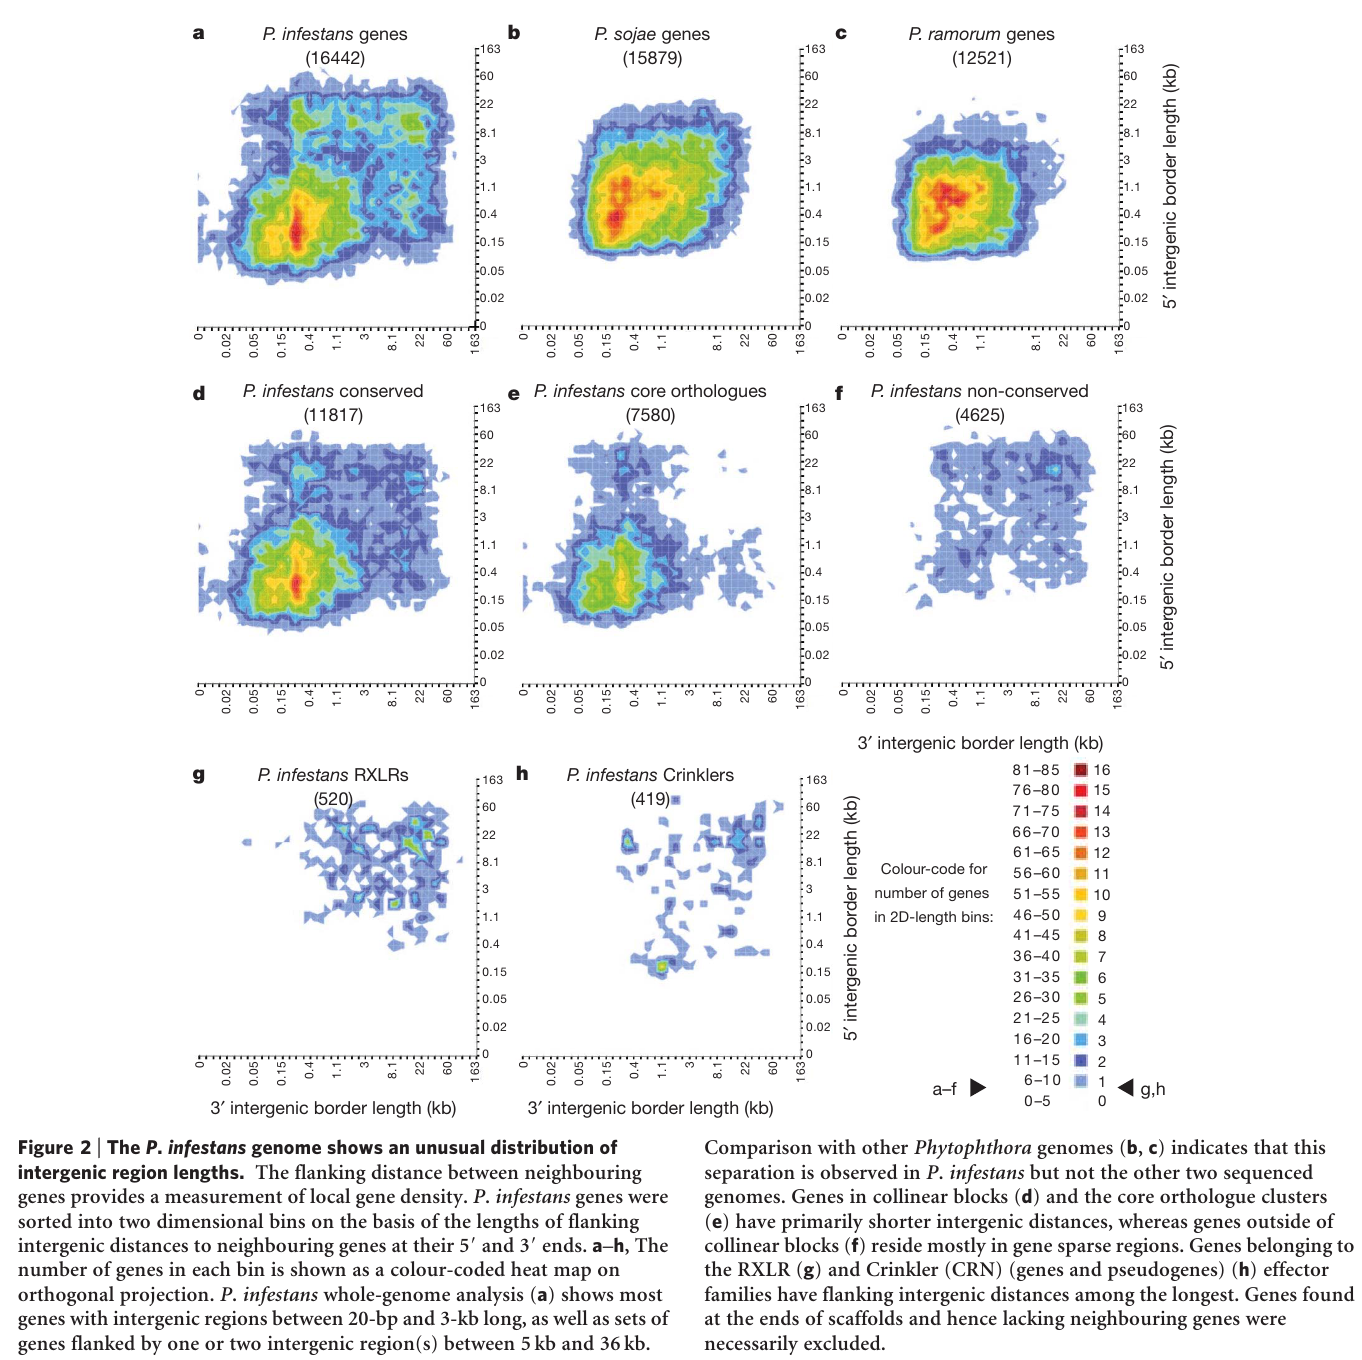
\includegraphics[width=\textwidth]{haas_blight_2009-fig2}
    \caption{
        Haas (2009) \cite{haas_genome_2009}
    }
  \end{figure}

  \begin{figure}[h!]
    \centering
    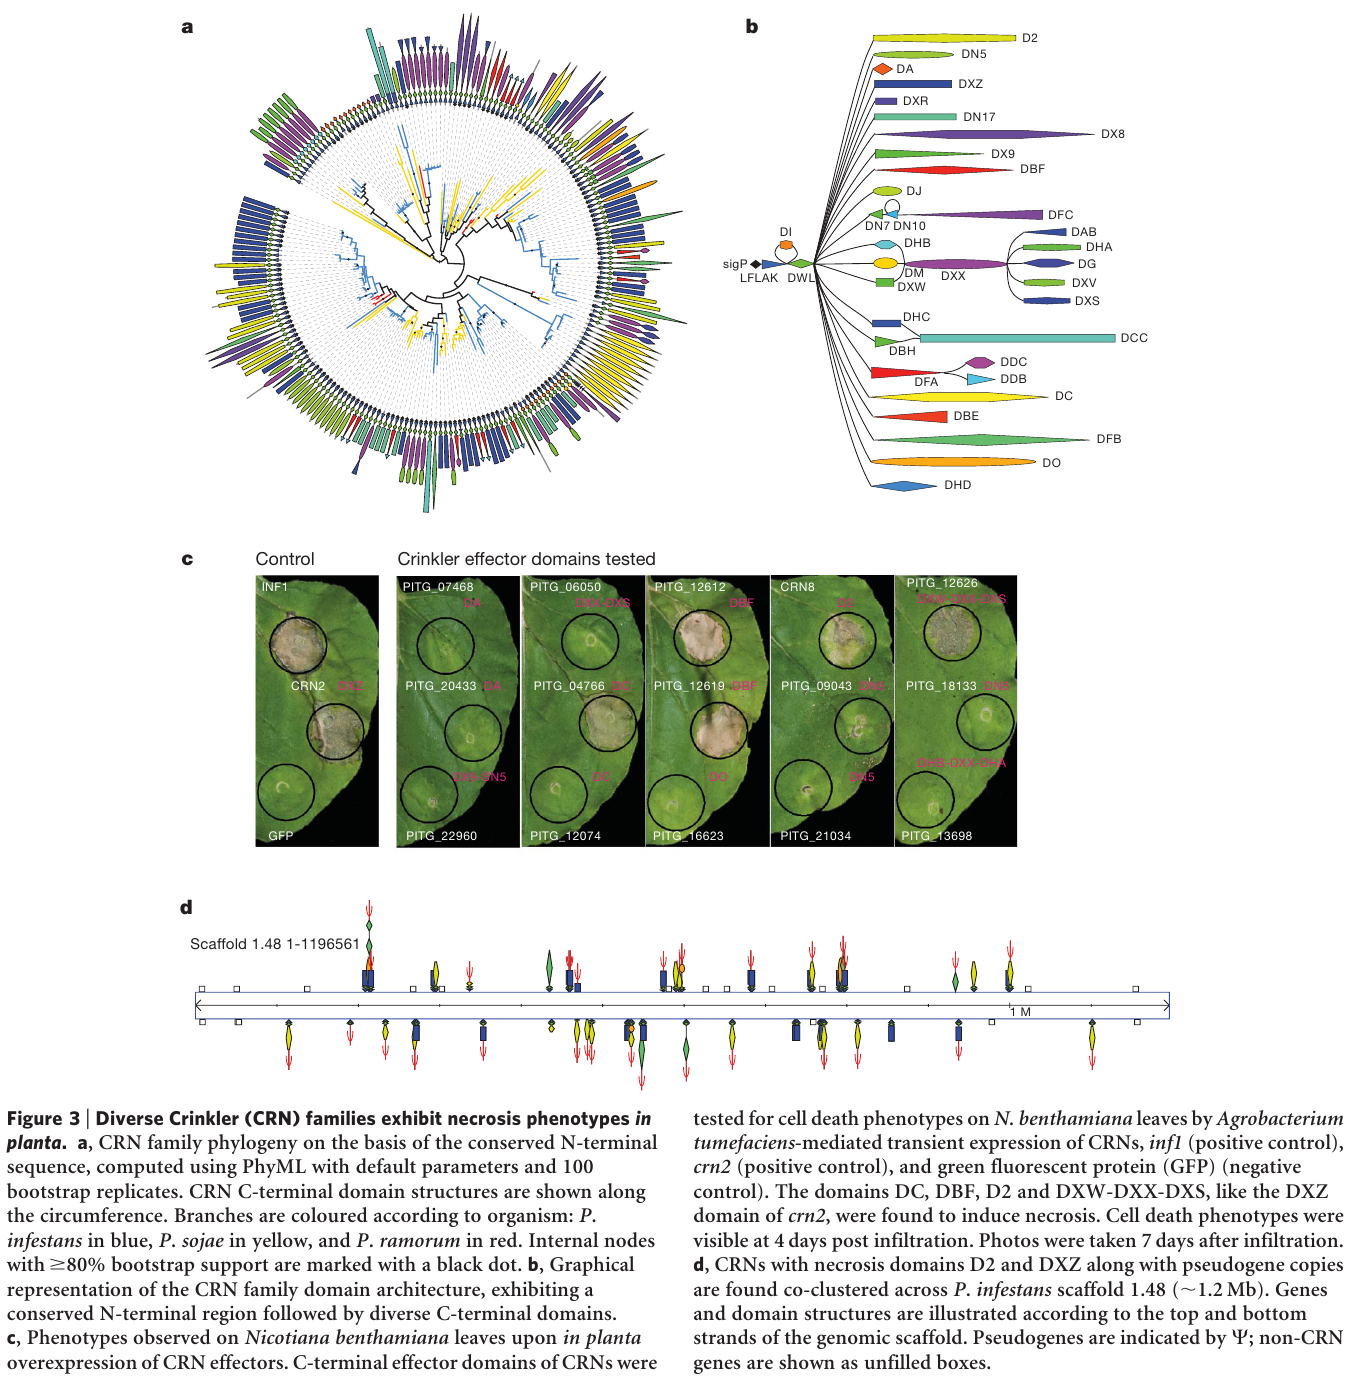
\includegraphics[width=\textwidth]{haas_blight_2009-fig3}
    \caption{
        Haas (2009) \cite{haas_genome_2009}
    }
  \end{figure}

  \FloatBarrier

\subsection{18 Dothideomycetes Fungi genomes}

  Citation \cite{ohm_diverse_2012}

  \begin{figure}[h!] \centering
    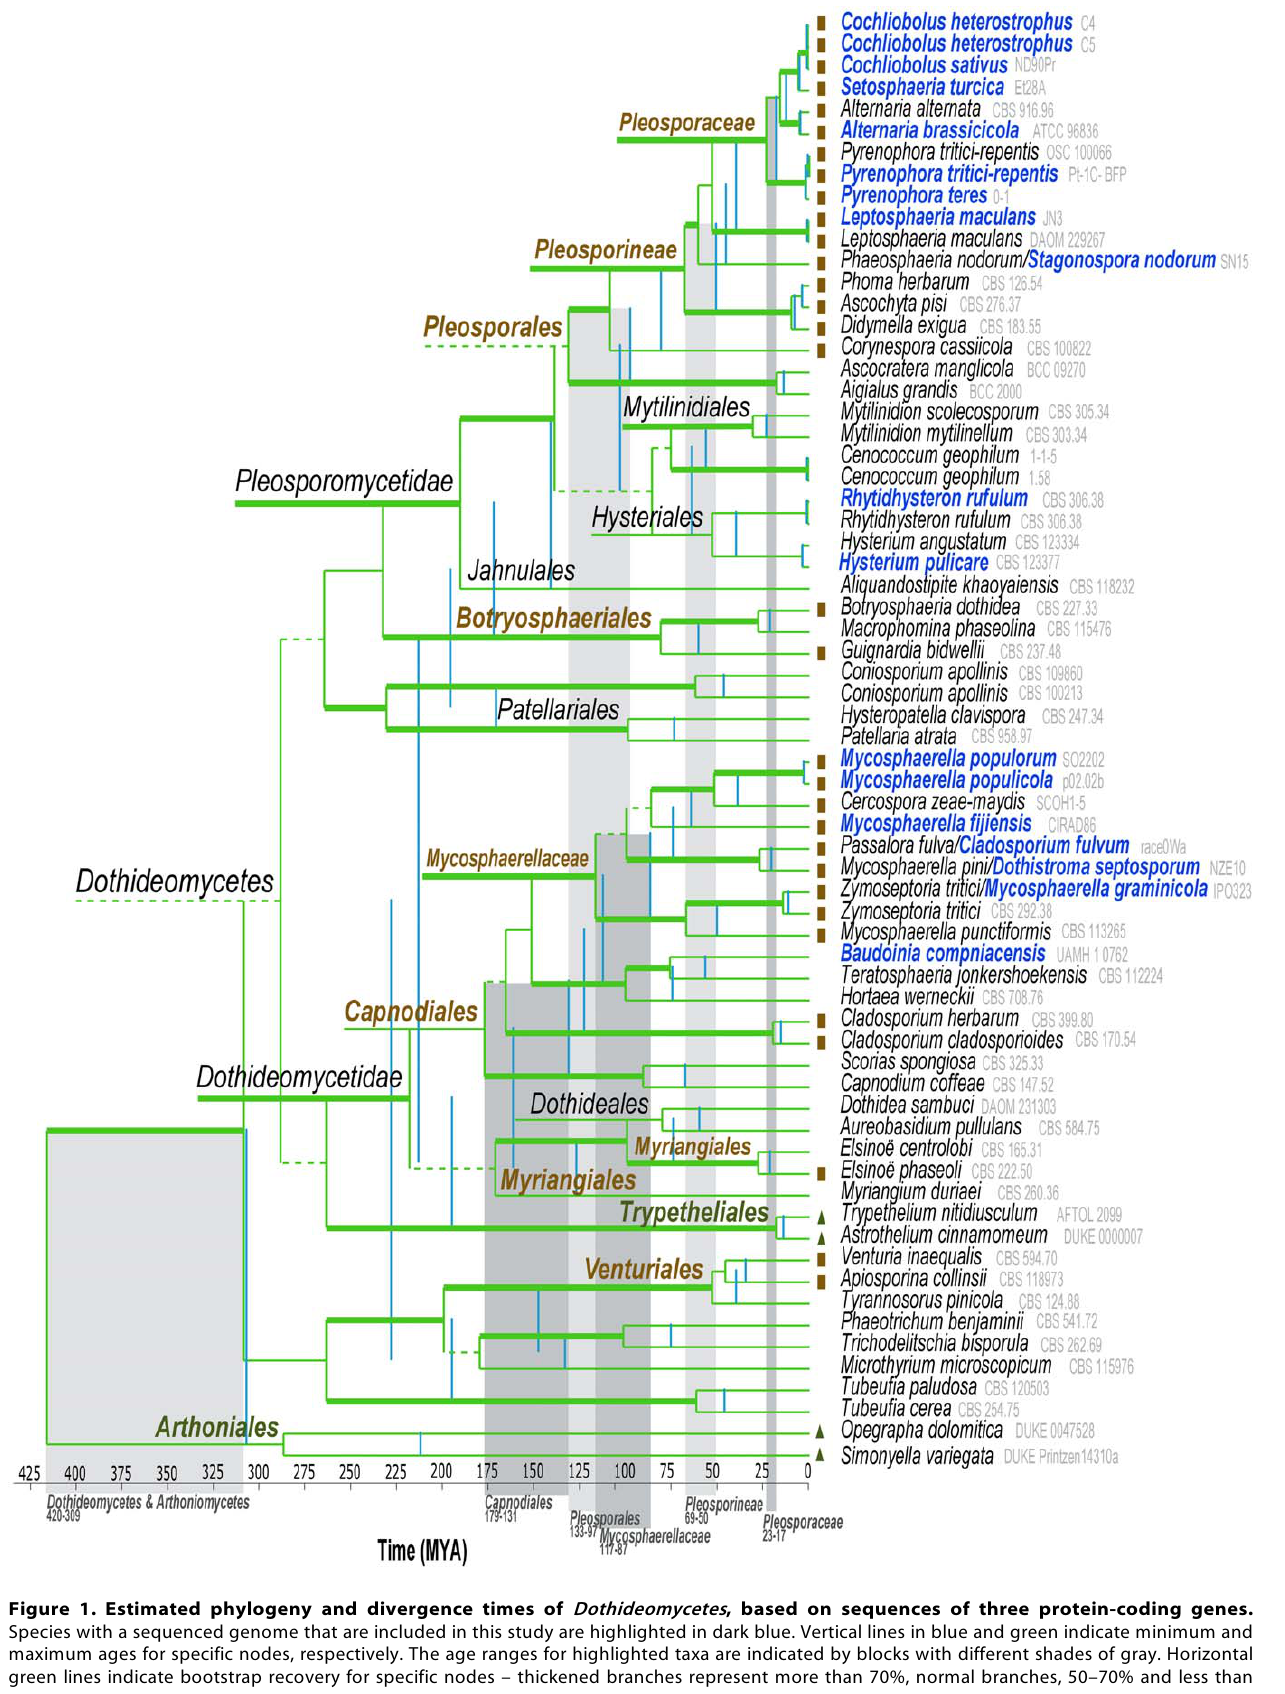
\includegraphics[height=0.7\textheight]{ohm_18fungi_2012-fig1}
  \end{figure}

  \begin{figure}[h!] \centering
    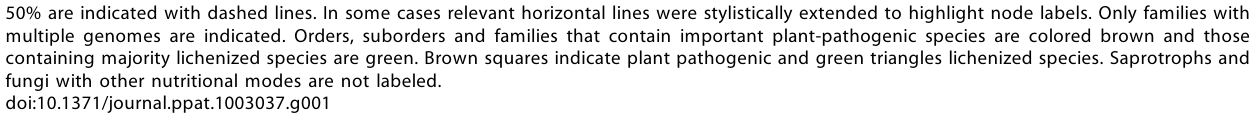
\includegraphics[width=0.7\textwidth]{ohm_18fungi_2012-fig1b}
    \caption{Ohm (2012) \cite{ohm_diverse_2012}}
  \end{figure}

  \begin{figure}[h!] \centering
    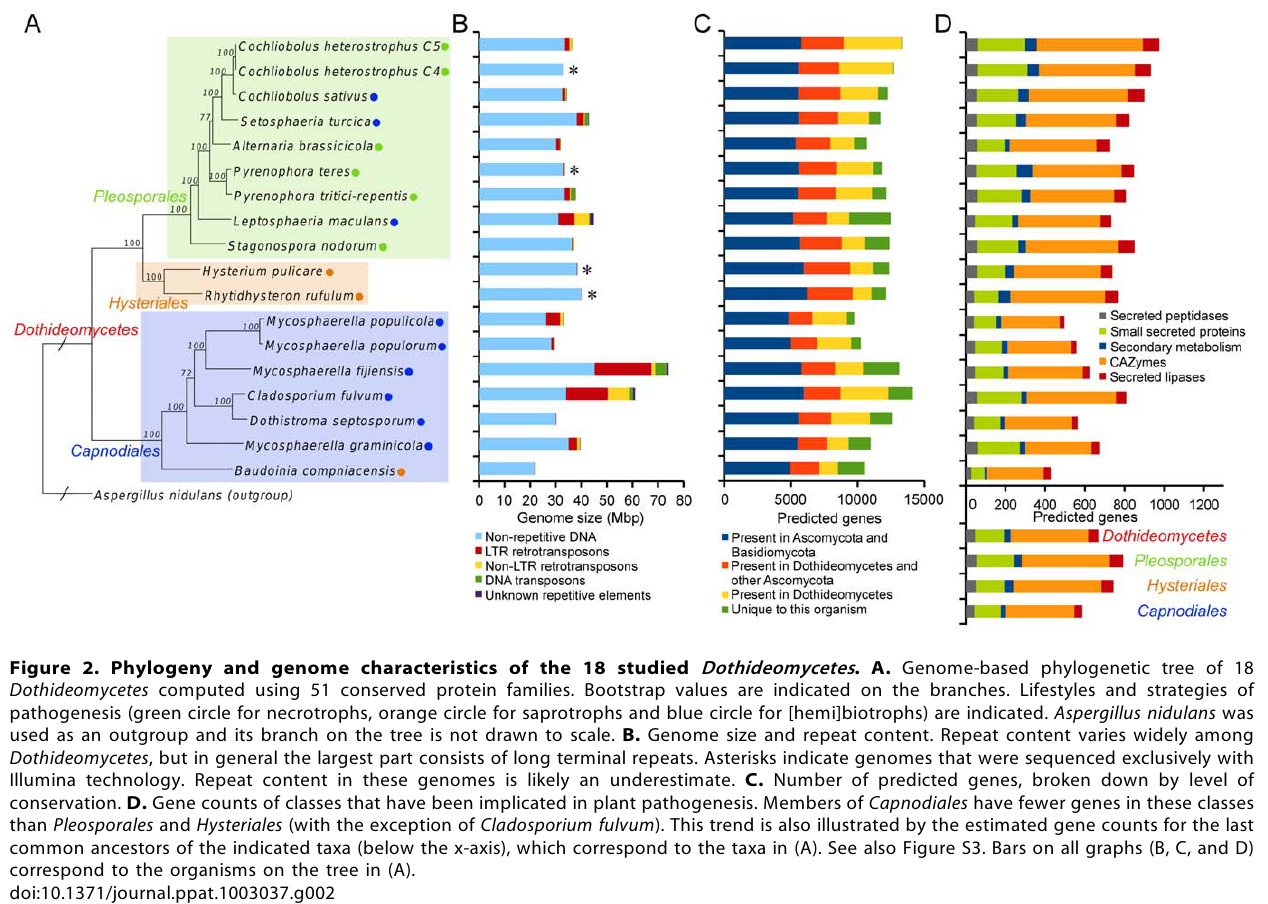
\includegraphics[width=\textwidth]{ohm_18fungi_2012-fig2}
    \caption{Ohm (2012) \cite{ohm_diverse_2012}}
  \end{figure}

  \begin{figure}[h!] \centering
    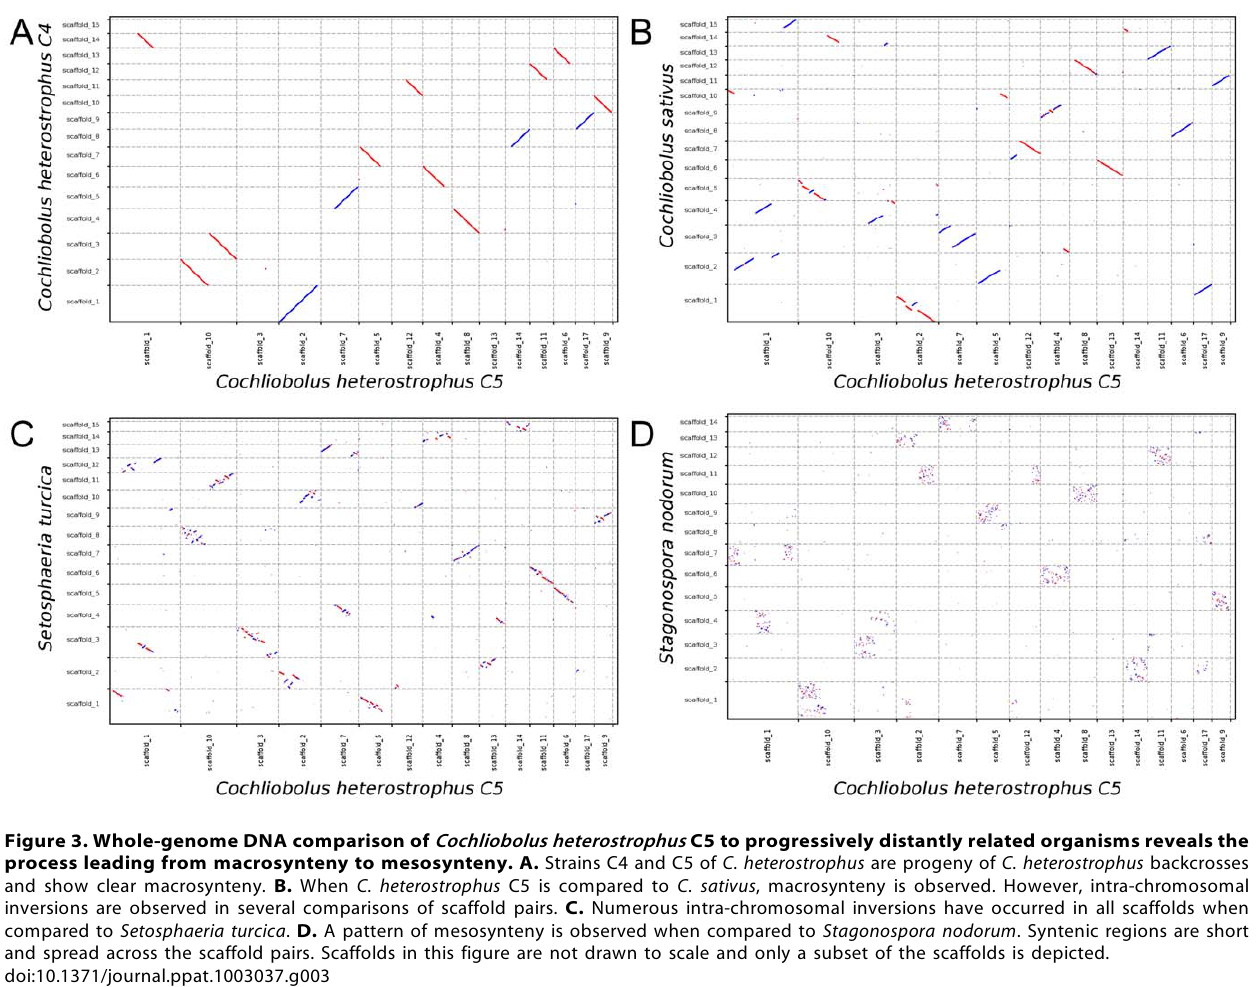
\includegraphics[width=\textwidth]{ohm_18fungi_2012-fig3}
    \caption{Ohm (2012) \cite{ohm_diverse_2012}}
  \end{figure}

  \FloatBarrier

\subsection{Setosphaeria fungi genome}

  Citation \cite{wu_setosphaeria_2013}

  \begin{figure}[h!] \centering
    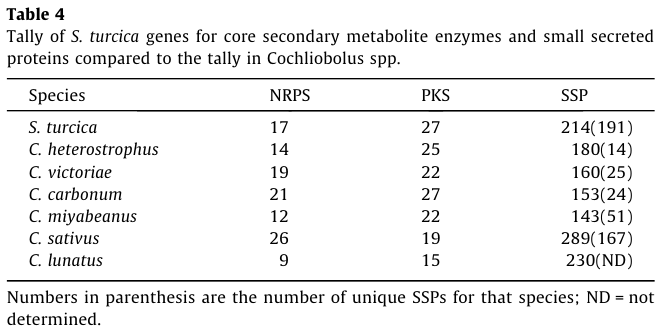
\includegraphics[width=0.6\textwidth]{wu_setosphaeria_2013-t1}
    \caption{Wu (2013) \cite{wu_setosphaeria_2013}}
  \end{figure}

  ``As reported in (Condon et al., 2013), candidate SSPs in S. turcica and
  nine Cochliobolus isolates were identified by screening gene catalogs for
  proteins smaller than 200 amino acids, containing more than 2\% cysteine,
  secretion signals, and lacking transmem- brane domains (Table 4).
  Cross-genome comparisons were made based on all vs. all reciprocal best hit
  analysis with an 80\% similarity cutoff (species-unique in parentheses).
  Note that both hemibio- trophs in this comparison, S. turcica and C.
  sativus, contained more strain unique SSPs than necrotrophs.'' pp. 4 (see
  table)

  \FloatBarrier
\subsection{Spanu (2010): Powdery Mildew \textit{ Blumeria graminis f.sp. hordei}}

  Citation \cite{spanu_genome_2010}

  No RIP, 64\% TE composition. Genes are clustered in little islands in the transposon sea.


  ``In addition to >1350 paralog copies of the previously described atypical
  avirulence genes AVRk1 and AVRa10 (11), we predicted 248 Blumeria proteins with
  a signal peptide (SP) but lacking any transmembrane domain and BLAST (Basic
  Local Alignment Search Tool) hit outside the mildews, thus representing
  candidates for secreted effector proteins (CSEPs) (12). The CSEPs have
  distinctive features (table S6) and show great sequence diversity with few
  members grouping in small families (Fig. 3A). We noted no obvious clustering of
  CSEPs within the Blumeria contigs. Approximately 80\% harbor a recently
  identified N-terminal tripeptide motif, termed “YxC,” (13), that typically
  occurs within the first 30 amino acids after the predicted SP cleavage site.
  Searches in the E. pisi and G. orontii genomes revealed that the vast majority
  of CSEPs are confined to Blumeria (Fig. 3A and table S6).  Thus, powdery mildew
  genomes preferentially harbor species- and/or tribe-specific innovations, which
  possibly evolved in the context of cospeciation with their plant hosts (11).
  Upon comparison of global gene expression in haustoria (Fig. 1C) and epiphytic
  structures (Fig. 1D), we observed preferential expression of the majority of
  the CSEPs (79\%) in haustoria (Fig. 3B), suggesting they have specific
  functions in biotrophic pathogenesis (14).'' pp. 4

  \begin{figure}[h!] \centering
    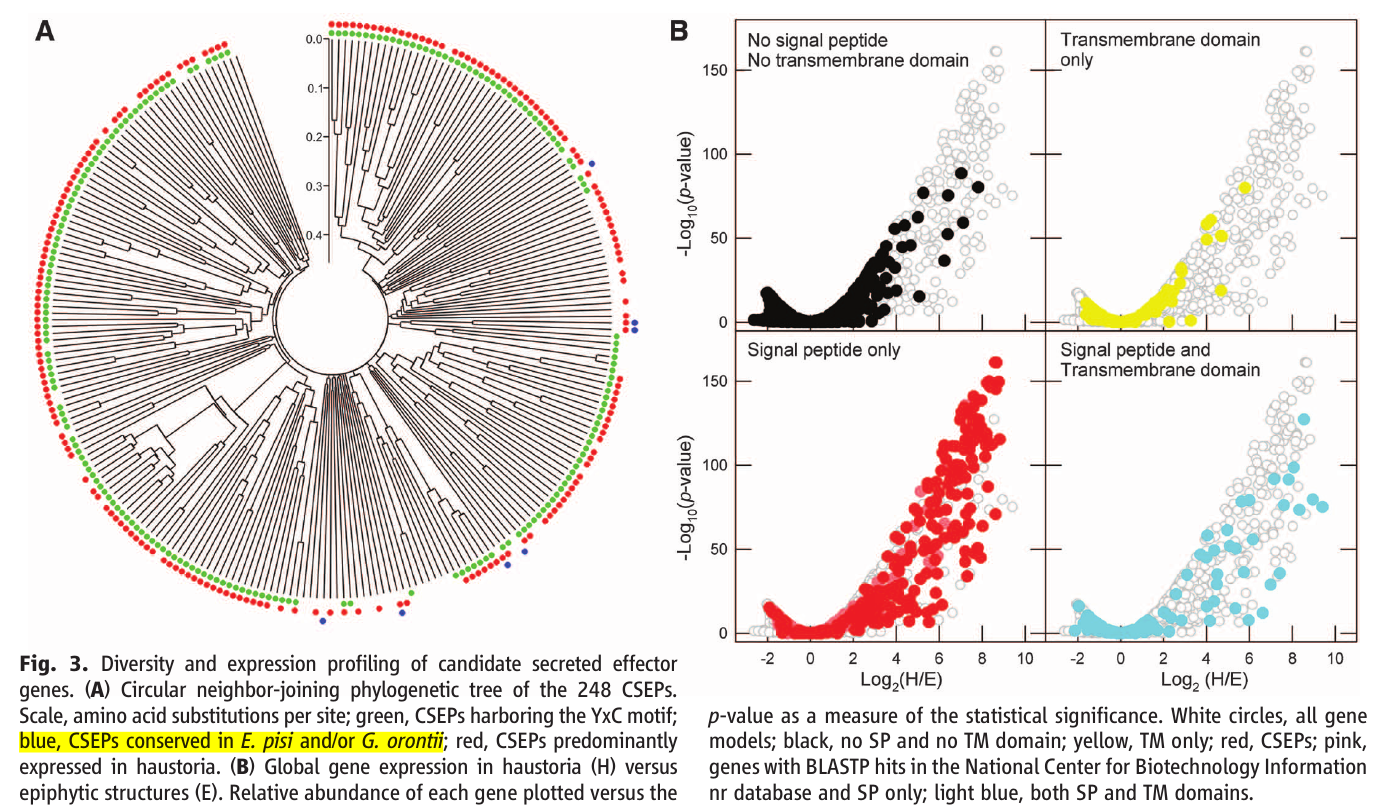
\includegraphics[width=\textwidth]{spanu_powder_2010-fig3}
    \caption{Spanu (2010) \cite{spanu_genome_2010}}
  \end{figure}
  \FloatBarrier

\subsection{Wicker (2013):Powdery Mildew \textit{ Blumeria graminis f.sp. tritici}}

  Citation \cite{wicker_wheat_2013}

  90\% transposable element (TE) composition

  The Blumeria graminis are divided into 8 \textit{formae speciales} that
  specifically infect a single host. tritici and hordei are estimated to be
  6.3 million years apart. 

  \begin{figure}[h!] \centering
    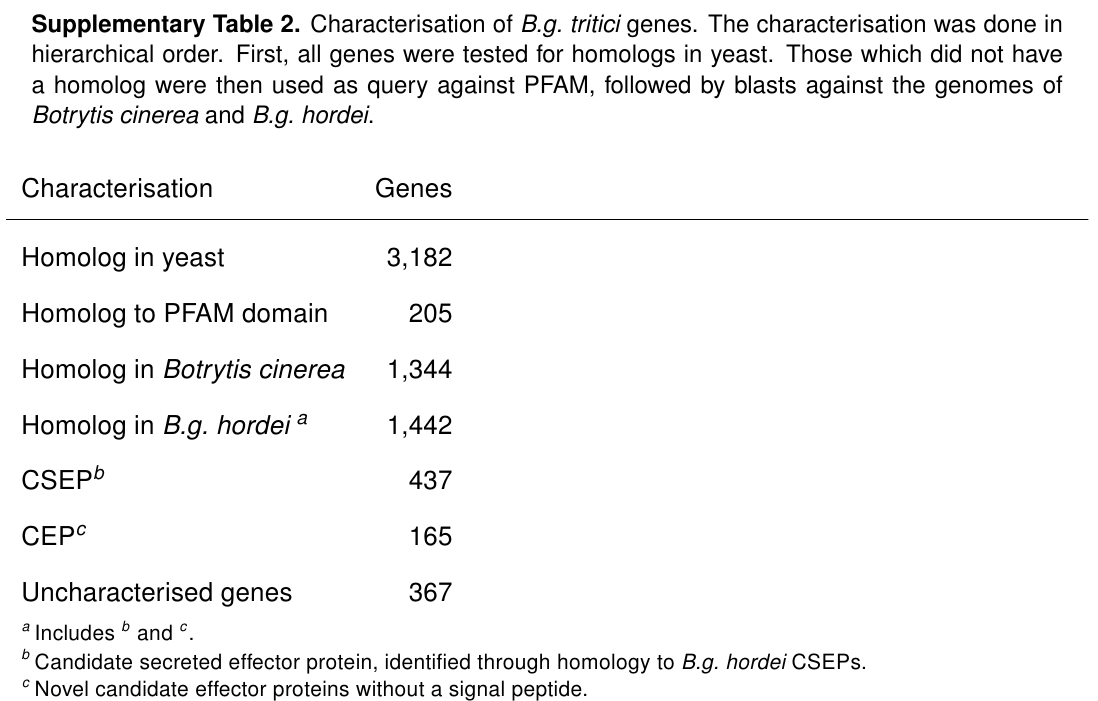
\includegraphics[width=0.7\textwidth]{wicker-rust-2013-suptab2}
    \caption{Wicker (2013) \cite{wicker_wheat_2013} It seems they didn't do thier own search for CSEPs}
  \end{figure}
  \FloatBarrier

  \begin{figure}[h!] \centering
    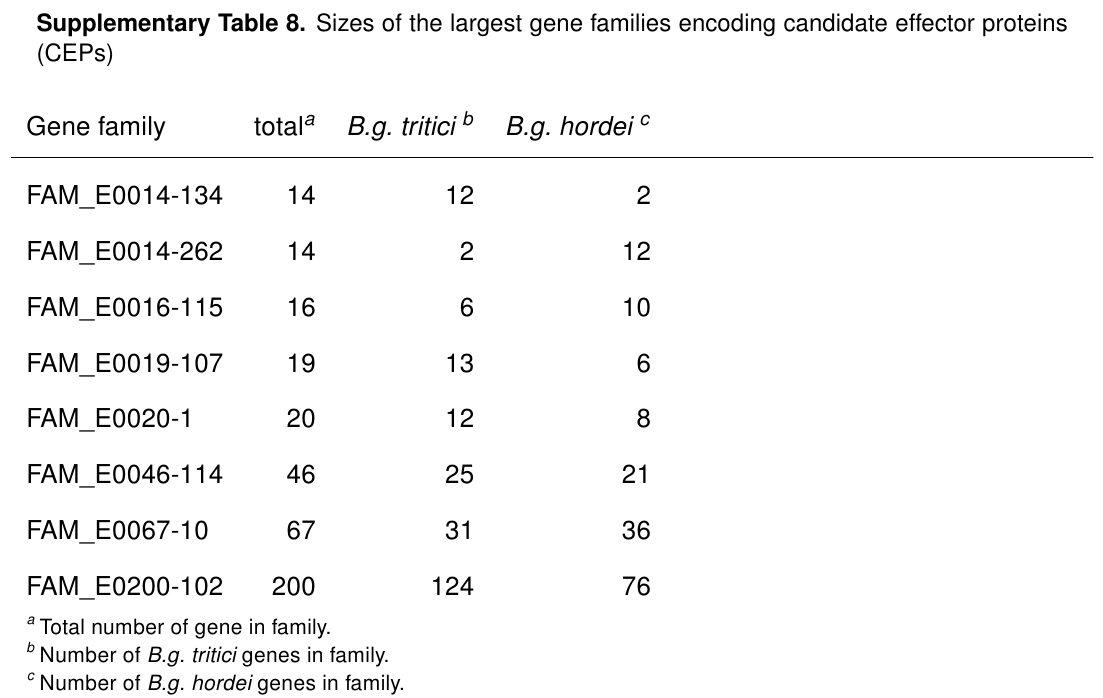
\includegraphics[width=0.7\textwidth]{wicker-rust-2013-suptab8}
    \caption{Wicker (2013) \cite{wicker_wheat_2013} }
  \end{figure}
  \FloatBarrier

  This is a shit paper. They didn't search for their own CSEPs in tritici,
  rather they identified CSEPs by looking for homologs in hordei.  They found
  437 CSEPs, while in hordei there are 248. So clearly there are major
  differences. But they didn't address this. Also they failed to mention
  which hordei CSEPs where \textit{not} present in tritici. So all we know is
  that at least one family of CSEPs is shared between the two sp.

  28\% of its genes had no homolog in Botrytis cinerea, seperate by 110 million years (TimeTree)

  Another annoying thing is that they find 92\% of the genes in tritici have
  a homolog in hordei. There conclusion is that the gene complement of the
  two subspecies is almost the same. In what universe is 8\% difference in
  gene content at a subspecies level \textit{almost the same}?

\subsection{Schnable (2009) B73 Maize}
  Citation \cite{schnable_b73_2009}

  \begin{figure}[h!] \centering
    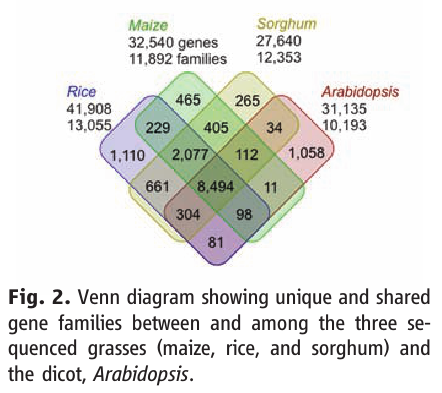
\includegraphics[width=0.3\textwidth]{schnable-maize-fig2}
    \caption{Schnable (2009) \cite{schnable_b73_2009}}
  \end{figure}
  \FloatBarrier

\section{Methods}

\subsection{Orphan origin classification}

  \subsubsection{duplicate}

    blastp or orphan genes against other coding genes in the focal species
    \cite{sun_identification_2015}. Use transitive property: if there is a
    match, and the paralog is not an orphan, assume duplication/divergence
    model. 

  \subsubsection{de novo}

    tBLASTn against nearby species. If there is a hit (50\% identity and 50\%
    coverage), and the hit is disrupted in all, classify as de novo. Manual
    checking of disruption status \cite{sun_identification_2015}.

  \subsubsection{TE}

    BLASTn against TE database (e-value cutoff of 1e-5)
    \cite{sun_identification_2015}.

\subsection{Mukherjee analysis of \textit{Leishmania major} (2015)}

  \cite{mukherjee_elucidating_2015}


  \begin{quote}

    To identify orphan gene models which are restricted to the Leishmania
    genus, we used a systematic way based on homology search. First, BLASTP
    followed by TBLASTN filtering approach ($E<10^5$ and use of low-complexity
    filters) was used against NCBI nr databases. Additionally, to further
    screen for similarity between sequences we employed Position-Specific
    Iterated BLAST (PSI-BLAST) ( Altschul et al., 1997) that can detect weaker
    homologous relationships that would otherwise be missed by the standard
    BLAST algorithms.

  \end{quote}

  The use of tBLASTn has the advantage of finding possible coding homologs of
  what would otherwise be misclassified as orphans. However, it would also
  misclassify \textit{any} true orphan that retains similarity to its
  precursor.

\subsection{Abrusan method}

Citation \cite{abrusan_integration_2013}

\textbf{Context} Orphans into networks, testing Carvunis

\textbf{Organism} Yeast

\textbf{Phylostratigraphy Procedure} 50 aa cutoff. 11 strata, 0 as Carvunis' unnanotated
genes, 1 as yeast annotated orphans, etc. Followed Carvunis methods. Time
estimates based on TimeTree.

\textbf{Protein Structure} PSSpred without homology search, since this
would introduce bias

\textbf{Aggregation propensity} Predicted with Tango

\textbf{Simulated Mutagenesis} Based on Schaefer's procedure
\cite{schaefer_protein_2010}. 1\% of the residues mutated in each of 70
steps. Mutations were introduced in context specific manner with csbuild
tool of CS-BLAST suite. At each step the secondary structure was predicted
and the percentage of sites with conserved structure was calculated.
Results were averaged for each gene across 5 replicates.

\subsection{Neme method}

Citation \cite{neme_phylogenetic_2013}

\textbf{Context} Metazoan de novo genes

\textbf{Organism} Mouse; a little human, zebrafish and stickleback

\textbf{Procedure} BLASTP(e-3) all mouse Ensembl 66 proteins against nr
database. For ps12 EST and Trace data were included in tBLASTn(e-15).
Phylostratiphy as normal.

\subsection{Hahn method}

Citation \cite{hahn_gene_2007}

\textbf{Context} 12 Drosophila genomes

\textbf{General Method} Clustering

\textbf{Notes} D. melanogaster seems to have ~2\% orphan composition. The
other genomes seem to have 10-30\% \cite{clark_evolution_2007}. Hahn
suspects this is an artefact of the overly lenient ab initio prediction
software. So he removes from the analysis all putative genes that are
unique to a single species. He calculates the percentage of Drosophila
specific genes, but since he circumsized the flange we can't really his
results to other orphan analyses. 

\textbf{Extinction} Hahn wasn't looking for, or interested in, orphans. His
focus was gene family dynamics. A very interesting result of his paper was
an estimate of family extinction. ``2,220 of the 11,434 families inferred
to have been present in the Drosophila MRCA have had such an extinction
event along at least one lineage'' pp. 7. This is something that has not
been researched nearly enough in the orphan context. If new genes are
constantly appearing, and proteome size is in equilibrium, then extinction
must be common as well. This introduces the idea of extinction
phylostratigraphy, the analysis of lineage-specific extinction events. The
technique will be more complicated than genesis phylostratigraphy since it
will require consideration of paralogs.

\subsection{Wu method}

Citation \cite{wu_novo_2011}

\textbf{Context} Finding human de novo genes

\textbf{General Method} Homology, synteny, RNA-seq, proteomics

\textbf{Details} Began with BLASTP(e-10) of all primate genomes. Removed
any proteins or splicing variants shorter than 100 amino acids (out 584).
Removed human proteins that lacked start or stop codons (weird, why were
they annotated as proteins?) (out 352). Searched these for orthologs with
BLAT against chimp and orangatan UCSC datavase. Removed all proteins for
which no homologous genomic region could be found. Removed candidates with
paralogs. Removed all if their genomic homologous region had a suitable
ORF. BLASTed remainder against mRNA database (to check for transcription)
and proteomic database (PRIDE and PeptideAtlas) to check for experimental
proof of protein product. This resulted in 27 proteins. They then ran genes
removed from the previous ann2tations, finding 33 additional true de novo
genes.

\subsection{Yang method}

Citation \cite{yang_genome-wide_2013}

\textbf{Context} Species specific and teleost specfic genes

\textbf{Organism} Zebrafish

\textbf{General method} Homology, manual

\textbf{Details} See figure.

\cfig{scale=0.2}{yang_zebra_method}{Yang \textit{et al.} orphan identification method}

\subsection{Toll-Reira Orphan Domain}

Citation \cite{toll-riera_emergence_2013}

\textbf{Context} Identify orphan domains in humans

\textbf{General Method} HMM

\textbf{Notes} Used PFAMs collection of domain-specific HMMs to identify
domains in all human genes. Classified domains by age group base on their
representation in 15 Eukaryotic species.
\subsection{Murphy Murine de novo genes}

Citation \cite{murphy_novo_2012}

\textbf{Context} Search for rat and mouse de novo genes

\textbf{General Method} BLAST

\textbf{Input} Rat and mouse annotated proteins (Ensembl v56)

\textbf{Procedure} BLASTP(e-3) rat-vs-mouse to identify orphans. BLASTN
rat-vs-mouse, keeping only candidates with a non-genic match (50\% coverage
and 70\% identity). Remove candidates with ortholog in non-murine species
via Ensembl compara database. Searched for potentially unannotated
protein-coding genes in opposite murine (tBLASTn to locate putative ORFs,
if translated ORF containing match aligns to at least 50\% and matches
60\%, then remove this gene). Remove an candidate lacking ATG start codon
or having an intron less than 18 bases in length. Used UniGene and Peptide
Atlas and Pride to confirm that the candidates are transcribed and
translated. BLASTed against GenBank (e-3 and 50\% coverage).

\textbf{Further Procedure} Searched for enabling mutations.

\subsection{Synteny based methods}

\subsubsection{Zhang, 2010}

Citation \cite{zhang_chromosomal_2010}

\textbf{Context} Male-biased genes in mammals

\textbf{General Method} BLAST and synteny

\textbf{Input} 


\section{Observations from my data}

\begin{enumerate}
\item There are about 700,000 non-genic ORFs

% ngORF, orphan, non-orphan comp table
\begin{table}[ht]
\centering
\begin{tabular}{|l|l|l|}
    \hline
    {} & \multicolumn{1}{c|}{Protein Length} & \multicolumn{1}{c|}{GC Percent}\\ 
    {} & (min, 25\%, \textbf{median}, 75\%, max) & (min, 25\%, \textbf{median}, 75\%, max) \\
    \hline
    ngORF & (10, 13, \textbf{19}, 29, 463) & (0.0152, 0.278, \textbf{0.322}, 0.368, 0.756) \\ 
    Orphan & (16, 43, \textbf{57}, 89, 1220) & (0.248, 0.396, \textbf{0.431}, 0.465, 0.69) \\ 
    Non-Orphan & (24, 214, \textbf{356}, 528, 5390) & (0.282, 0.423, \textbf{0.441}, 0.463, 0.657) \\ 
    \hline
\end{tabular}
\end{table}

There are 8,249 ngORFs (about 0.011\%) that have both lengths and GC\% within
the mid-50\% range of the orphan genes. Most likely, the de novo orphans
originate from such ORFs. There may be orphan nursuries, high GC islands, in
which orphan genes frequently appear. 

Orphans are a little \textbf{less} structured than ngORFs. All the trends I
have tested agree with those of Carvunis \cite{carvunis_proto-genes_2012} and
others. Orphans are likely just as important in plants as they have been
demonstrated to be in metazoans and yeast.

\end{enumerate}



\section{Case studies}

\subsection{False orphans}

\subsubsection{AT3G53370.2 - splicing artifact}

AT3G53370.2 is classified as an orphan according to blastp (threshold 1e-5).
However the model AT3G53370.1 is classified as Embryophyta-specific.

\begin{verbatim}
 >AT3G53370.2
 MDGEDFAG                                        KNLPPRKKKPVSKKKLKREKLKQGVPVPGE
 >AT3G53370.1
 MDGEDFAG KAAAEAKGLNPGLIVLLVVGGPLLVFLIANYVLYVYAQ KNLPPRKKKPVSKKKLKREKLKQGVPVPGE
\end{verbatim}

HMM-based methods are sensative enough to detect the similarity, however.
HHBlits and HMMER easily detect its similarity to other S1FA DNA binding
domains.

\subsection{Orphan gene families}

\subsubsection{Panther: PTHR31420}

Also pfam-domain DUF3287

\begin{verbatim}
 model         pfam-A  pfam-B  stratum
 AT3G32150.1   0       0       21     
 AT3G32190.1   1       0       21     
 AT3G33293.1   0       0       21     
 AT4G06583.1   0       1       21     
 AT4G07932.1   0       1       21     
 AT4G08097.1   0       0       21     
 AT5G35603.3   0       1       21     
 AT5G33898.1   0       1       21     
 AT3G30220.1   0       1       20     
 AT3G32160.1   0       1       20     
 AT3G32180.1   0       1       20     
 AT4G06583.2   0       1       20     
 AT4G07740.1   0       1       20     
 AT5G35603.1   0       1       20     
 AT5G35603.2   0       1       20     
 AT2G11010.1   0       1       18     
 AT3G30230.1   0       0       18     
 AT3G43148.1   1       0       18     
 AT4G06688.1   0       0       18     
 AT3G43150.1   0       1       14     
 AT5G32590.1   1       0       11     
\end{verbatim}


\section{Other} 
\subsection{Questions about this review}

    \begin{enumerate} 
        \item What do people need to know
            about orphans?  
            \begin{enumerate} 
                \item What they are 
                \item Where and how many they are 
                \item Explain modern flange 
                \item How they are identified 
                \item Where they come from 
                \item Why they are important 
                \item Significance to ID 
            \end{enumerate} 
        \item What has already been covered by other reviewers?  
        \item What unique insights does this paper offer?  
        \begin{enumerate} 
            \item Examples of functional orphans (QQS) 
            \item Case study in Arabidopsis thaliana 
            \item Words of caution about the interpretation of orphan studies and
                phylostratigraphy 
            \item Explain difficulties of comparing orphan studies
                
        \end{enumerate} 
        \item What questions does this paper pose?
            \begin{enumerate} 
                \item How much does annotation affect phylostratification?  
            \end{enumerate} 
        \item How will this paper benefit the community?  
        \begin{enumerate} 
            \item Provide a context for interpreting orphan studies 
            \item Describes potential problems that need to be addressed 
            \item Describe the conditions wherein studies of orphans is possible 
        \end{enumerate} 
    \end{enumerate}

\subsection{More general stuff}

    Assume all genes are of equal age. How would we describe what we see?

    The ``orphan'' genes would simply be genes that evolve extremely quickly. Their
    rapid evolution explains their low codon and amino acid specialization.

    \begin{enumerate}
        \item Are plant ngORFs widely transcribed? Translated?
        \item How many ngORFs are actually translated? How many ought to be
            annotated as genes? Are essential?
        \item Are orphan selfish? Rising to become essential so fast, suspicious?
    \end{enumerate}

    Where would I expect, prior to looking at any evidence, new genes to appear?
    Anywhere evolution must work rapidly. In plants I would expect genes related to
    defense against pathogens or pests to evolve quickly.
\subsection{At as orphan model}

Great opportunity to study sub-species level orphan trends. This will allow
evolutionary properties to be studied. It will allow identification of the At
orphans that are under purifying or positive selection, aiding in
identification of true orphans. It will allow the regulation development to be
studied in great detail. It will allow estimates of orphan genesis and
extinction rates. For example, 18 genomes \cite{gan_multiple_2011}, 1001
genomes \cite{weigel_1001_2009}, Sweden genomes \cite{long_massive_2013}.

\subsection{Non-coding Orphans}

Identification of a bunch of functional ncRNA orphans in At
\cite{riano-pachon_orphan_2005}

miRNA orphans are also common, as seen in Drosophila \cite{zhang_age-dependent_2010}

\subsection{PUFs and POFs}

\subsubsection{Definitions}

    \textbf{PUFs - Liberal definition}: proteins with no known function OR
    sequence homology to any such proteins. Anything similar to something
    with function is assigned that function.

    \textbf{PUFs - Conservative definition}: proteins with lack of experimental
    support of specific function. Everything is asigned functionality based
    on its own merit.

    \textbf{POFs}: Proteins with Obscure Features

\subsubsection{Horan (2008) Annotating Genes of Known and Unknown Function
by Large-Scale Coexpression Analysis}

    Citation \cite{horan_annotating_2008}

    Uses three methods for identifying PUFs: GO terms (32-38\%), BLASTP
    against SwissProt, HMMpfam against PFAM.

\subsubsection{Gollery (2006) What makes species unique? The
contribution of proteins with obscure features}

    Citation \cite{gollery_what_2006}

\section{Statistical methods}

\subsection{Reproducibile research}

    There was a recent series in nature about the repoducibility issues faced
    in science
    (\href{http://www.nature.com/news/reproducibility-1.17552}{here}).

    A review on the lack of reproducibility of p-values
    \cite{halsey_fickle_2015}. P-values are a random variables. We would never
    report a single measurement without a standard deviation. Similarly we
    should not report p-values without mentioning the power of the study.


\addcontentsline{toc}{section}{References}
\bibliographystyle{bibsty}
\bibliography{notes}

\end{document}
